\documentclass[11pt]{article}
\usepackage{graphicx, tikz-cd, float} % Required for inserting images
\usepackage{amsmath, amssymb, amsthm, amsfonts, siunitx, physics, gensymb, chemfig}
\AtBeginDocument{\RenewCommandCopy\qty\SI}
\usepackage[version=4]{mhchem}
\usepackage[most,many,breakable]{tcolorbox}
\usepackage{xcolor, fancyhdr, varwidth}
\usepackage[Glenn]{fncychap}
%Options: Sonny, Lenny, Glenn, Conny, Rejne, Bjarne, Bjornstrup
\usepackage{hyperref, cleveref}
\usepackage{icomma, enumitem} %comma as decimal and continue enumerate with [resume]
\usepackage{booktabs}
%%%%%%%%%%%%%%%%%%%%%%%%%%%%%%
% SELF MADE COLORS
%%%%%%%%%%%%%%%%%%%%%%%%%%%%%%
\definecolor{myg}{RGB}{56, 140, 70}
\definecolor{myb}{RGB}{45, 111, 177}
\definecolor{myr}{RGB}{199, 68, 64}
\definecolor{mytheorembg}{HTML}{F2F2F9}
\definecolor{mytheoremfr}{HTML}{00007B}
\definecolor{mylenmabg}{HTML}{FFFAF8}
\definecolor{mylenmafr}{HTML}{983b0f}
\definecolor{mypropbg}{HTML}{f2fbfc}
\definecolor{mypropfr}{HTML}{191971}
\definecolor{myexamplebg}{HTML}{F2FBF8}
\definecolor{myexamplefr}{HTML}{88D6D1}
\definecolor{myexampleti}{HTML}{2A7F7F}
\definecolor{mydefinitbg}{HTML}{E5E5FF}
\definecolor{mydefinitfr}{HTML}{3F3FA3}
\definecolor{notesgreen}{RGB}{0,162,0}
\definecolor{myp}{RGB}{197, 92, 212}
\definecolor{mygr}{HTML}{2C3338}
\definecolor{myred}{RGB}{127,0,0}
\definecolor{myyellow}{RGB}{169,121,69}
\definecolor{myexercisebg}{HTML}{F2FBF8}
\definecolor{myexercisefg}{HTML}{88D6D1}
%%%%%%%%%%%%%%%%%%%%%%%%%%%%%%%%%%%%%%%%%%%%%%%%%%%%%%%%%%%%%%%%%%%%%%
% Box environments for theorems and problems
%%%%%%%%%%%%%%%%%%%%%%%%%%%%%%%%%%%%%%%%%%%%%%%%%%%%%%%%%%%%%%%%%%%%%
\setlength{\parindent}{1cm}
%================================
% Question BOX
%================================
\makeatletter
\newtcbtheorem{question}{Opgave}{enhanced,
	breakable,
	colback=white,
	colframe=myb!80!black,
	attach boxed title to top left={yshift*=-\tcboxedtitleheight},
	fonttitle=\bfseries,
	title={#2},
	boxed title size=title,
	boxed title style={%
			sharp corners,
			rounded corners=northwest,
			colback=tcbcolframe,
			boxrule=0pt,
		},
	underlay boxed title={%
			\path[fill=tcbcolframe] (title.south west)--(title.south east)
			to[out=0, in=180] ([xshift=5mm]title.east)--
			(title.center-|frame.east)
			[rounded corners=\kvtcb@arc] |-
			(frame.north) -| cycle;
		},
	#1
}{def}
\makeatother
%================================
% DEFINITION BOX
%================================

\newtcbtheorem[]{Definition}{Definition}{enhanced,
	before skip=2mm,after skip=2mm, colback=red!5,colframe=red!80!black,boxrule=0.5mm,
	attach boxed title to top left={xshift=1cm,yshift*=1mm-\tcboxedtitleheight}, varwidth boxed title*=-3cm,
	boxed title style={frame code={
					\path[fill=tcbcolback]
					([yshift=-1mm,xshift=-1mm]frame.north west)
					arc[start angle=0,end angle=180,radius=1mm]
					([yshift=-1mm,xshift=1mm]frame.north east)
					arc[start angle=180,end angle=0,radius=1mm];
					\path[left color=tcbcolback!60!black,right color=tcbcolback!60!black,
						middle color=tcbcolback!80!black]
					([xshift=-2mm]frame.north west) -- ([xshift=2mm]frame.north east)
					[rounded corners=1mm]-- ([xshift=1mm,yshift=-1mm]frame.north east)
					-- (frame.south east) -- (frame.south west)
					-- ([xshift=-1mm,yshift=-1mm]frame.north west)
					[sharp corners]-- cycle;
				},interior engine=empty,
		},
	fonttitle=\bfseries,
	title={#2},#1}{def}
\newtcbtheorem[]{definition}{Definition}{enhanced,
	before skip=2mm,after skip=2mm, colback=red!5,colframe=red!80!black,boxrule=0.5mm,
	attach boxed title to top left={xshift=1cm,yshift*=1mm-\tcboxedtitleheight}, varwidth boxed title*=-3cm,
	boxed title style={frame code={
					\path[fill=tcbcolback]
					([yshift=-1mm,xshift=-1mm]frame.north west)
					arc[start angle=0,end angle=180,radius=1mm]
					([yshift=-1mm,xshift=1mm]frame.north east)
					arc[start angle=180,end angle=0,radius=1mm];
					\path[left color=tcbcolback!60!black,right color=tcbcolback!60!black,
						middle color=tcbcolback!80!black]
					([xshift=-2mm]frame.north west) -- ([xshift=2mm]frame.north east)
					[rounded corners=1mm]-- ([xshift=1mm,yshift=-1mm]frame.north east)
					-- (frame.south east) -- (frame.south west)
					-- ([xshift=-1mm,yshift=-1mm]frame.north west)
					[sharp corners]-- cycle;
				},interior engine=empty,
		},
	fonttitle=\bfseries,
	title={#2},#1}{def}

\newtcbtheorem{theo}%
    {Theorem}{}{theorem}
\newtcolorbox{prob}[1]{colback=red!5!white,colframe=red!50!black,fonttitle=\bfseries,title={#1}}
%================================
% NOTE BOX
%================================

\usetikzlibrary{arrows,calc,shadows.blur}
\tcbuselibrary{skins}
\newtcolorbox{note}[1][]{%
	enhanced jigsaw,
	colback=gray!20!white,%
	colframe=gray!80!black,
	size=small,
	boxrule=1pt,
	title=\textbf{Note:},
	halign title=flush center,
	coltitle=black,
	breakable,
	drop shadow=black!50!white,
	attach boxed title to top left={xshift=1cm,yshift=-\tcboxedtitleheight/2,yshifttext=-\tcboxedtitleheight/2},
	minipage boxed title=1.5cm,
	boxed title style={%
			colback=white,
			size=fbox,
			boxrule=1pt,
			boxsep=2pt,
			underlay={%
					\coordinate (dotA) at ($(interior.west) + (-0.5pt,0)$);
					\coordinate (dotB) at ($(interior.east) + (0.5pt,0)$);
					\begin{scope}
						\clip (interior.north west) rectangle ([xshift=3ex]interior.east);
						\filldraw [white, blur shadow={shadow opacity=60, shadow yshift=-.75ex}, rounded corners=2pt] (interior.north west) rectangle (interior.south east);
					\end{scope}
					\begin{scope}[gray!80!black]
						\fill (dotA) circle (2pt);
						\fill (dotB) circle (2pt);
					\end{scope}
				},
		},
	#1,
}

%%%%%%%%%%%%%%%%%%%%%%%%%%%%%%%%%%%%%%%%%%%%%%%%%%%%%%%%%%%%%%%%%
% SELF MADE COMMANDS
%%%%%%%%%%%%%%%%%%%%%%%%%%%%%%
\newcommand{\sol}{\setlength{\parindent}{0cm}\textbf{\textit{Løsning:}}\setlength{\parindent}{1cm}}

\theoremstyle{definition}
\newtheorem{defi}{Definition}[section]
\newtheorem{postu}{Postulat}
%%%%%%%%%%%%%%%%%%%%%%%%%%%%%%%%%
\usepackage[tmargin=2cm,rmargin=1in,lmargin=1in,margin=0.85in,bmargin=2cm,footskip=.2in]{geometry}\pagestyle{fancy}
\setlength{\headheight}{13.6pt}
\lhead{Minrui Kevin Zhou 2.b}
\usepackage[round]{natbib} %%Or change 'round' to 'square' for square backers
%\renewcommand\refname{Litteraturliste}
%\renewcommand\abstractname{Resumé}
%\renewcommand\contentsname{Indholdsfortegnelse}
%\renewcommand\figurename{Figur}
\usepackage{setspace} %%Enables \doublespacing command for double linespacing
\usepackage[danish]{babel}

\title{SRO}
\author{Kevin Zhou, 2.b}
\date{\today}

\begin{document}
%----------------------------------------------------------------------------------------
%	TITLE PAGE
%----------------------------------------------------------------------------------------

\begin{titlepage} % Suppresses displaying the page number on the title page and the subsequent page counts as page 1
	\newcommand{\HRule}{\rule{\linewidth}{0.5mm}} % Defines a new command for horizontal lines, change thickness here
	
	\center % Centre everything on the page
	
	%------------------------------------------------
	%	Headings
	%------------------------------------------------
	
	\textsc{\LARGE Virum Gymnasium}\\[1.5cm] % Main heading such as the name of your university/college
	
	\textsc{SRO}\\[0.5cm] % Major heading such as course name
	
	\textsc{Fysik og Kemi}\\[0.5cm] % Minor heading such as course title
	
	%------------------------------------------------
	%	Title
	%------------------------------------------------
	
	\HRule\\[0.4cm]
	
	{\huge\bfseries Applikationer af Bohrs atommodel og Lambert-Beers lov i spektroskopi}\\[0.4cm] % Title of your document
	
	\HRule\\[1.5cm]
	
	%------------------------------------------------
	%	Author(s)
	%------------------------------------------------
	
	\begin{minipage}{0.4\textwidth}
		\begin{flushleft}
			\large
			\textit{Forfatter}\\
			 \textsc{Minrui Kevin Zhou} % Your name
		\end{flushleft}
	\end{minipage}
	~
	\begin{minipage}{0.4\textwidth}
		\begin{flushright}
			\large
			\textit{Vejledere}\\
			\textsc{Carsten Andreasen}\\ % Supervisor's name
      \textsc{Ole Vesterlund Nielsen}
		\end{flushright}
	\end{minipage}
	
	% If you don't want a supervisor, uncomment the two lines below and comment the code above
	%{\large\textit{Author}}\\
	%John \textsc{Smith} % Your name
	
	%------------------------------------------------
	%	Date
	%------------------------------------------------
	
	\vfill\vfill\vfill % Position the date 3/4 down the remaining page
	
	{\large\today} % Date, change the \today to a set date if you want to be precise
	
	%------------------------------------------------
	%	Logo
	%------------------------------------------------
	
	%\vfill
	
\includegraphics[width=0.3\textwidth]{VG.png}\\[1cm] % Include a department/university logo - this will require the graphicx package
	 
	%----------------------------------------------------------------------------------------
	
	\vfill % Push the date up 1/4 of the remaining page
	
\end{titlepage}

%----------------------------------------------------------------------------------------



\begin{abstract}
I denne opgave undersøger vi, hvordan Bohrs atommodel og Lambert-Beers lov kan appliceres med hensyn til spektroskopi.
Vi gør dette ved at kigge på emmision med hensyn til atomer og absorption med hensyn til molekyler.
Vi benytter Bohrs atommodel til at optage et spektrum af atomar hydrogen, som vi sammeligner med spektret for enkeltioniseret helium og dobbelt-ioniseret lithium.
Sammenfaldet mellem nogle af linjerne i spektrene for disse forklarer vi med Bohrs atommodel, der også kan bruges til at fortælle noget om hydrogenlignende atomer.
Vi bruger Lambert-Beers lov til at bestemme koncentrationen af farvestofferne azorubin, sunset yellow og tartrazin i en Cuba Apricot Vodka vha. spektrofotometri.
  Disse får vi til at være henholdsvis $11,1 \;\unit{mg/L}$, $0,0593 \;\unit{mg/L}$ og $13,4 \;\unit{mg/L} $. 
\end{abstract}

\tableofcontents
\thispagestyle{empty}
\newpage

\section{Introduktion} \label{intro}
Ved at skyde fotoner på henholdsvis atomer og molekyler, kan man få informationer om dem.
Dette fortæller Bohrs atommodel og Lambert-Beers lov noget om.
I denne opgave viser vi, hvordan disse kan appliceres med hensyn til spektroskopi.
Vi ser både på emmision med hensyn til atomer og absorption med hensyn til molekyler.
Vi introducerer først Bohrs atommodel og derefter Lambert-Beers lov samt hvad absorbans er.
Herefter undersøger vi tre farvestoffer, som er i en Cuba Apricot Vodka, da disse er relevante i forhold til en af eksperimenterne.
Så benytter vi Bohrs atommodel til at optage et spektrum af atomar hydrogen, som vi sammeligner med spektret for enkeltioniseret helium og dobbelt-ioniseret lithium.
Til sidst bruger vi Lambert-Beers lov til at bestemme koncentrationen af farvestofferne azorubin, sunset yellow og tartrazin i en Cuba Apricot Vodka vha. spektrofotometri.

\section{Teori}
\subsection{Bohrs atommodel}
I Bohrs atommodel består atomet af en positivt ladet kerne, hvor der er negative elektroner, som bevæger sig rundt om den i baner.
Modellen tager udgangspunkt i to postulater.\footnote{\cite{Brydensholt2021}, side 300}
\begin{postu}
 Atomet kan kun eksistere i noigle ganske bestemte stationære tilstande. I hver af disse tilstande har atomet en bestemt energi. 
\end{postu}
En stationær tilstand er en tilstand, hvor atomet ikke mister energi.
\begin{postu}
  Ændringer fra en tilstand med energien $E_n$ til en anden med energien $E_m$ kan ske ved, at atomet enten emitterer eller absorberer en foton med energien
  \[
  h\cdot f=E_n-E_m
  \] 
  hvor $f$ er atomets frekvens og $h$ er Plancks konstant. 
\end{postu}
Ved at benytte disse postulater, kan man angiveligt komme frem til, at ligning \ref{eq:En} gælder for hydrogenatomet.\footnote{\cite{Brydensholt2021}, side 302}
\begin{equation}
\label{eq:En}
\begin{split}
  E_n=-\frac{h\cdot c\cdot R}{n^2}
\end{split}
\end{equation}
hvor $h$ er Plancks konstant, $c$ er lysets fart og $R$ er Rydberg-konstanten. 
Ved indsættelse af værdierner får vi
\[
E_n=\frac{-13,6 \;\unit{eV} }{n^2}
\] 
Bohrs model af hydrogenatomet kan også bruges til at forudsige spektrene for hydrogenlignende atomer.
Atlså ioner, der er atomer, som har fået alle undtagen en af elektronerne fjernet.
Da gælder ligning \ref{eq:hyd_lign}.\footnote{\cite{RiceUniversity2023}, se 6.52}
\begin{equation}
\label{eq:hyd_lign}
\begin{split}
  E_n=\frac{-13,6 \;\unit{eV} \cdot Z^2}{n^2}
\end{split}
\end{equation}
hvor $Z$ er atomnummeret. 

\subsection{Lambert-Beers lov}
Vi finder koncentrationen af farvestofferne i vodkaen ved at kigge på absorbansen.
Denne måles med et spektrofotometer, hvori vi har en lyskilde, der passerer en monokromator og derefter en kuvette med opløsningen, hvorefter en detektor måler lysets intensitet. 
Lysintensiteten måles først med det rene opløsningsmiddel i kuvetten og kaldes $I_0$.
Derefter måler vi lysintensiteten med opløsningen nede i kuvetten, som vi kalder for $I$.
Absorbansen, $A$, for opløsningen kan nu defineres.\footnote{\cite{Mygind2022}, side 184}
\begin{defi}[Absorbans]
  Lad $A(\lambda)$ være absorbansen for opløsningen ved bølgelængden $\lambda$ og lad $I$ være lysintensiteten efter passage af opløsningen.
Lad $I_0$ være lysintensiteten efter passage af det rene opløsningsmiddel. 
Så gælder der, at
\[
  A(\lambda)=\log_{10}\left(\frac{I_0}{I}\right).
\] 
\end{defi}
Det viser sig, at når opløsningen er fortyndet, så koncentrationen af det absorberende stof er realtivt lille, så absorbansen helst er mindre end 1, så er absorbansen proportional med den aktuelle stofmængdekoncentration af det absorberende stof, $[\text{stof}]$, og at absorbansen også er proportional med lysvejens længde $l$.\footnote{\cite{Mygind2022}, side 186}
Da gælder Lambert-Beers lov, som ses i ligning \ref{eq:Lamb}, hvor $\varepsilon_{\lambda}$ er den molære ekstinktionskoefficient, der afhængder af bølgelængden og det absorberende stof. 
\begin{equation}
\label{eq:Lamb}
\begin{split}
  A(\lambda)=\varepsilon_{\lambda} \cdot l \cdot [\text{stof}]
\end{split}
\end{equation}
I vores eksperiment angives koncentrationen af farvestofferne i $\unit{mg/L} $ og betegnes med $c(\text{farvestof})$.
Lysvejens længde ændres heller ikke, og bølgelængden er konstant.
Lambert-Beers lov kan derfor skrives som i ligning \ref{eq:Lamb2}.
For at se, hvorfor dette er tilfældet, bemærk at $$k_{\lambda}=\frac{\varepsilon_{\lambda}\cdot l}{M(\text{stof})}$$
\begin{equation}
\label{eq:Lamb2}
\begin{split}
  A(\lambda)=k_{\lambda}\cdot c(\text{stof})
\end{split}
\end{equation}
I en opløsning (som per definition er et homogent medium) med adskillige absorberende stoffer er absorbansbidragene for hvert enkelt absorberende stof additive.\footnote{\cite{Mayerhofer2019}, side 2749}
Det vil altså sige, at hvis en opløsning indeholder flere forskellige absorberende stoffer, så vil absorbansen for opløsningen være lig med summen af absorbanserne for opløsninger med de samme koncentrationer af de absorberende stoffer hver for sig.

\subsection{Azorubin, sunset yellow og tartrazin}
I vores Cuba Apricot Vodka er der tre forskellige absorberende stoffer.
Disse er de tre kunstige farvestoffer, som kaldes azorubin, sunset yellow og tartrazin.
Strukturformlerne for disse fra PubChem kan ses i \cref{fig:azo}, \cref{fig:sun} og \cref{fig:tar}.\footnote{\cite{PubChem2023,PubChem2023a,PubChem2023b}}
\begin{figure}[H]
\begin{center}
  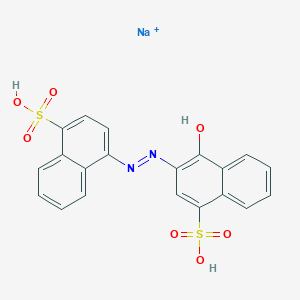
\includegraphics[scale=1]{azorubin.png}
\end{center}
\caption{Strukurformlen for azorubin}
\label{fig:azo}
\end{figure}

\begin{figure}[H]
\begin{center}
  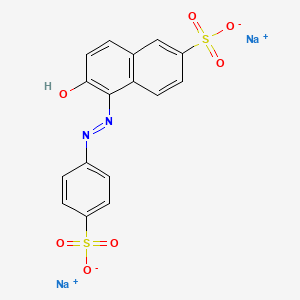
\includegraphics[scale=1]{sunset.png}
\end{center}
\caption{Strukturformlen for sunset yellow}
\label{fig:sun}
\end{figure}

\begin{figure}[H]
\begin{center}
  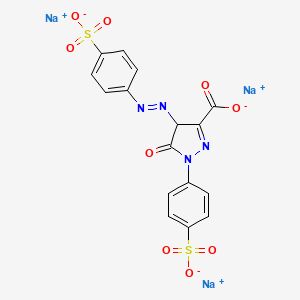
\includegraphics[scale=1]{tartrazin.png}
\end{center}
\caption{Strukturformlen for tartrazin}
\label{fig:tar}
\end{figure}
Generelt siger man, at et organisk stof er farvet, hvis der minimum er otte konjugerede dobbeltbindinger i molekylet.\footnote{\cite{Mygind2022}, side 179} 
Konjugerede dobbeltbindinger er dobbeltbindinger, hvorimellem der er præcis én enkeltbinding.
Da er det nemt at se, at der i hvert enkelt molekyle for de tre forskellige farvestoffer er mere end otte konjugerede dobbeltbindinger.
Chromofore grupper har også betydning for stoffernes farve.
De tre farvestoffer indeholder alle den chromofore gruppe azo, \ce{-N=N-}, og er derfor azofarvestoffer. 
Med hensyn til chromofore grupper, indholder tartrazin også en carbonylgruppe: 
\[
\chemfig{C(-[:135])(-[:225])(=[:0]O)}
\] 
Med hensyn til auxochrome grupper, der er farvemodificerende, indeholder azorubin og sunset yellow en hydroxygruppe, \ce{-OH}.

\section{Metode}
\subsection{Spektrum for atomar hydrogen}
Vi benyttede programmet LoggerPro til målingerne.
Dette blev gjort med et fotospektrometer og tilhørende lyslederkabel, der blev forbundet til vores PC med et USB-kabel.
Vi tændte vores udladningsrør med hydrogen i et mørkt rum som i \cref{fig:hydrogen}.
Derefter førte vi lyslederkablet tæt på udladningsrøret for at måle den relative intensitet mht. forskellige bølgelængder.
Til sidst tog vi et billede af hydrogenspektret gennem et gitter.
\begin{figure}[H]
\begin{center}
  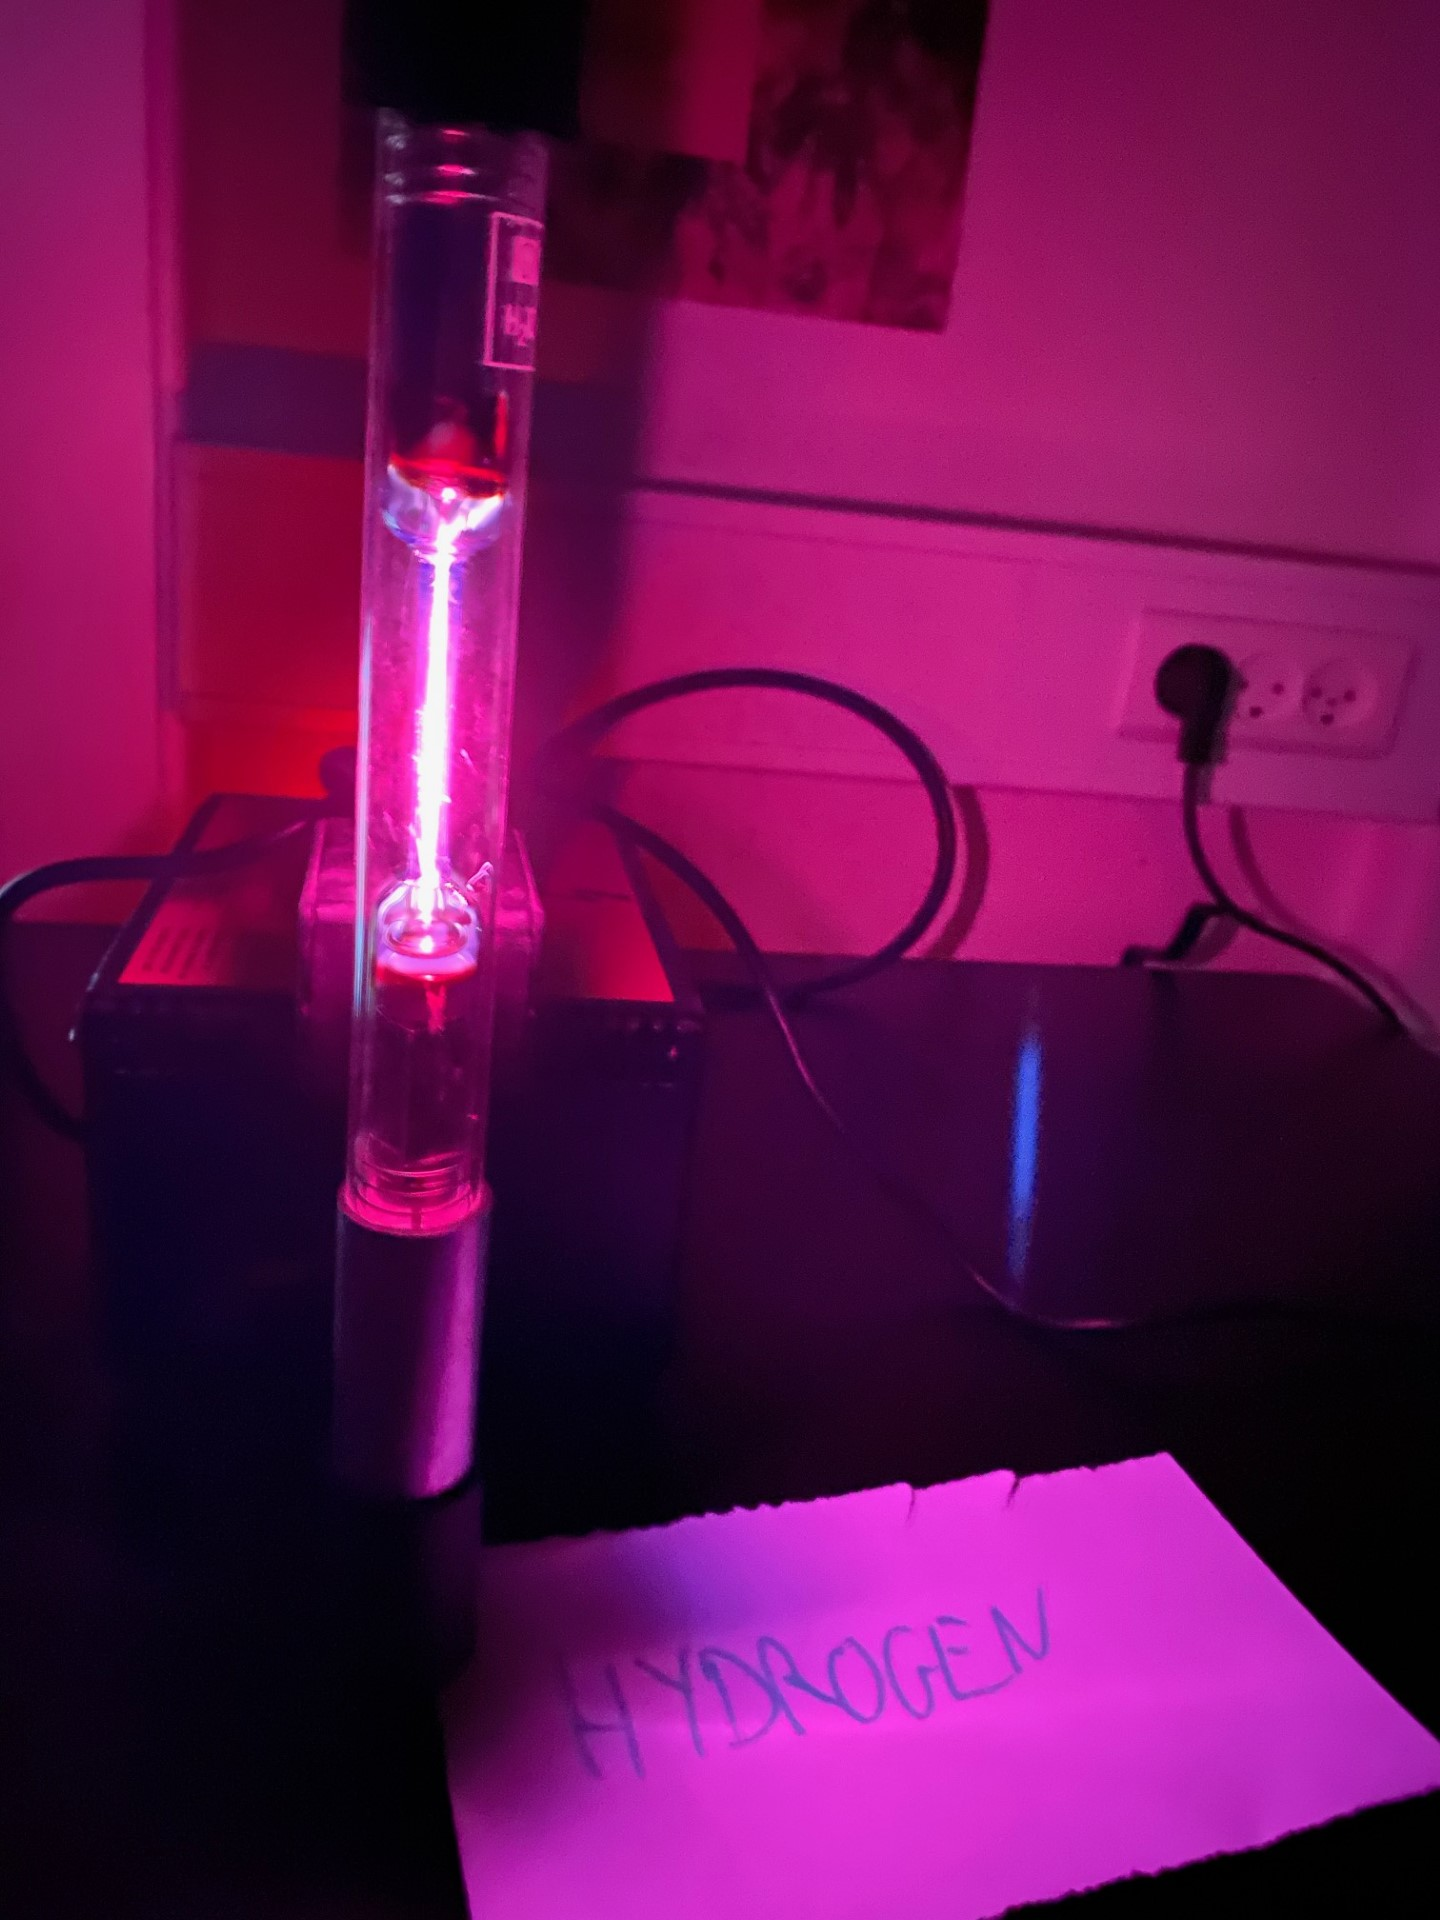
\includegraphics[width=0.7\textwidth]{hydrogen.jpeg}
\end{center}
\caption{Tændt udladningsrør med hydrogen}
\label{fig:hydrogen}
\end{figure}

\subsection{Bestemmelse af koncentrationerne af farvestoffer i vodka}
Først fremstillede vi fem standardopløsninger for hvert af de tre farvestoffer, henholdsvis azorubin, sunset yellow og tartrazin.
Dette illustreres af tabel \ref{tab:kon} og blev gjort i $25 \;\unit{mL}  $ målekolber, ved at fortynde vores stamopløsninger af farvestofferne, der havde koncentrationen $50,0 \;\unit{mg/L} $, med demineraliseret vand.
Standardopløsningerne for tartrazin ses i \cref{fig:stand}.
\begin{table}[H]
\centering
\begin{tabular}{@{}llllll@{}}
\toprule
\multicolumn{6}{c}{Farvestof}                                                                          \\ \midrule
Opløsning nr.                                               & 1     & 2     & 3      & 4      & 5      \\
  Volumen $50,0 \;\unit{mg/L} $ farvestof/\unit{mL} & 2,0 & 4,0 & 6,0 & 8,0 & 10,0 \\ 
$c(\text{farvestof})/\unit{mg/L}$ i $25\;\unit{mL}$ målekolbe & $4,0$ & $8,0$ & $12,0$ & $16,0$ & $20,0$ \\ \bottomrule
\end{tabular}
  \caption{Koncentrationen af farvestoffet i de numererede standardopløsninger}
  \label{tab:kon}
\end{table}
\begin{figure}[H]
\begin{center}
  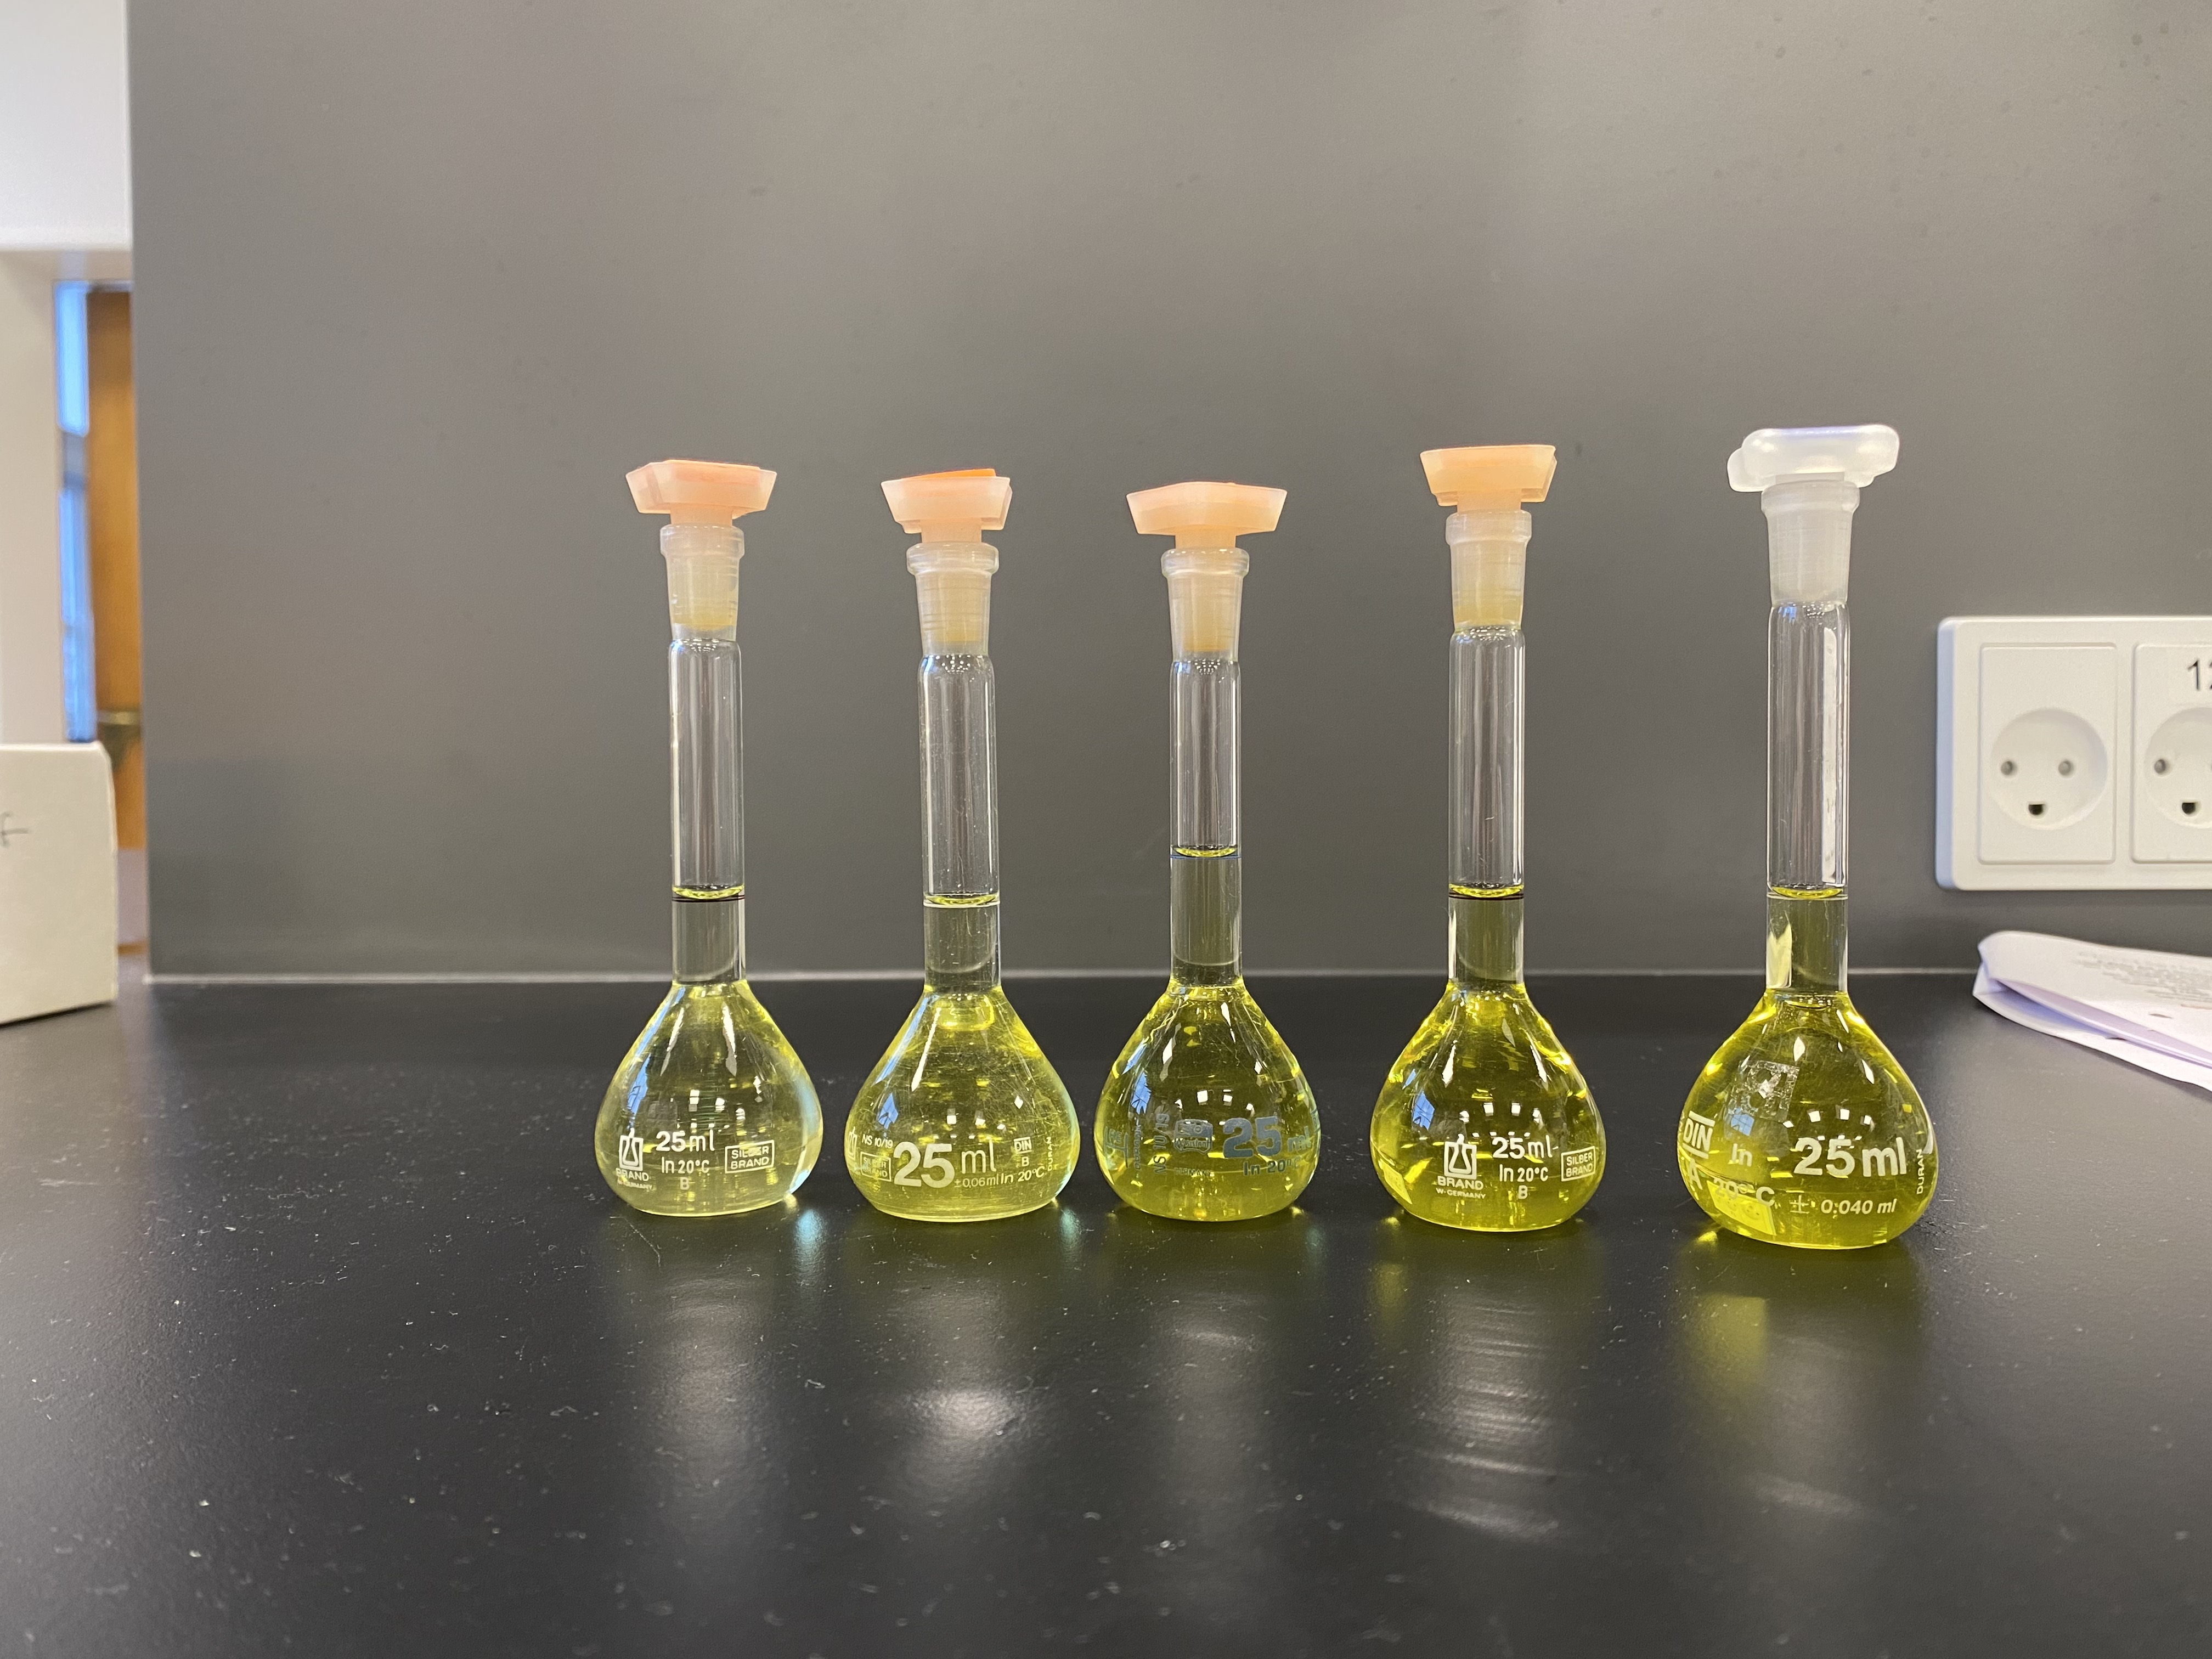
\includegraphics[width=0.7\textwidth]{standard.jpg}
\end{center}
\caption{Standardopløsningerne for tartrazin}
\label{fig:stand}
\end{figure}

Programmet LoggerPro blev brugt ved målingerne sammen med et spektrofotometer.
Vi tændte vores spektrofotometer og kalibrerede det med demineraliseret vand, da det er opløsningsmidlet.
Brugen af spektrofotometeret sker som på \cref{fig:spektro}, hvor kuvetten sættes ned i spektrofotometeret med en pipettespids for at fastgøre denne. 
Vi fyldte derefter en kuvette op med opløsning nr. 5 for hvert af de tre farvestoffer og optog et arbsorptionsspektrum.
Absorptionsspektret for tartrazin ses i \cref{fig:absorption}.
Dernæst kunne vi bestemme bølgelængden for hver af de tre farvestoffer, hvor absorbansen er maksimal. 
Disse fremgår af tabel \ref{tab:abs}.

For hver af de fem standardopløsninger for de tre forskellige farvestoffer målte vi så absorbanserne ved de tre bølgelængder, hvor absorbansen er maksimal for deres respektive farvestof.
Standardkurverne for tartrazin kan ses i \cref{fig:stand_kurve}

Til sidst fykdte vi en kuvette op med "Cuba Apricot Vodka", som ses i \cref{fig:vodka}.
Vi målte så absrobanserne ved de samme tre bølgelængder, hvor absorbansen er maksimal for de tre forskellige farvestoffer. 
\begin{figure}[H]
\begin{center}
  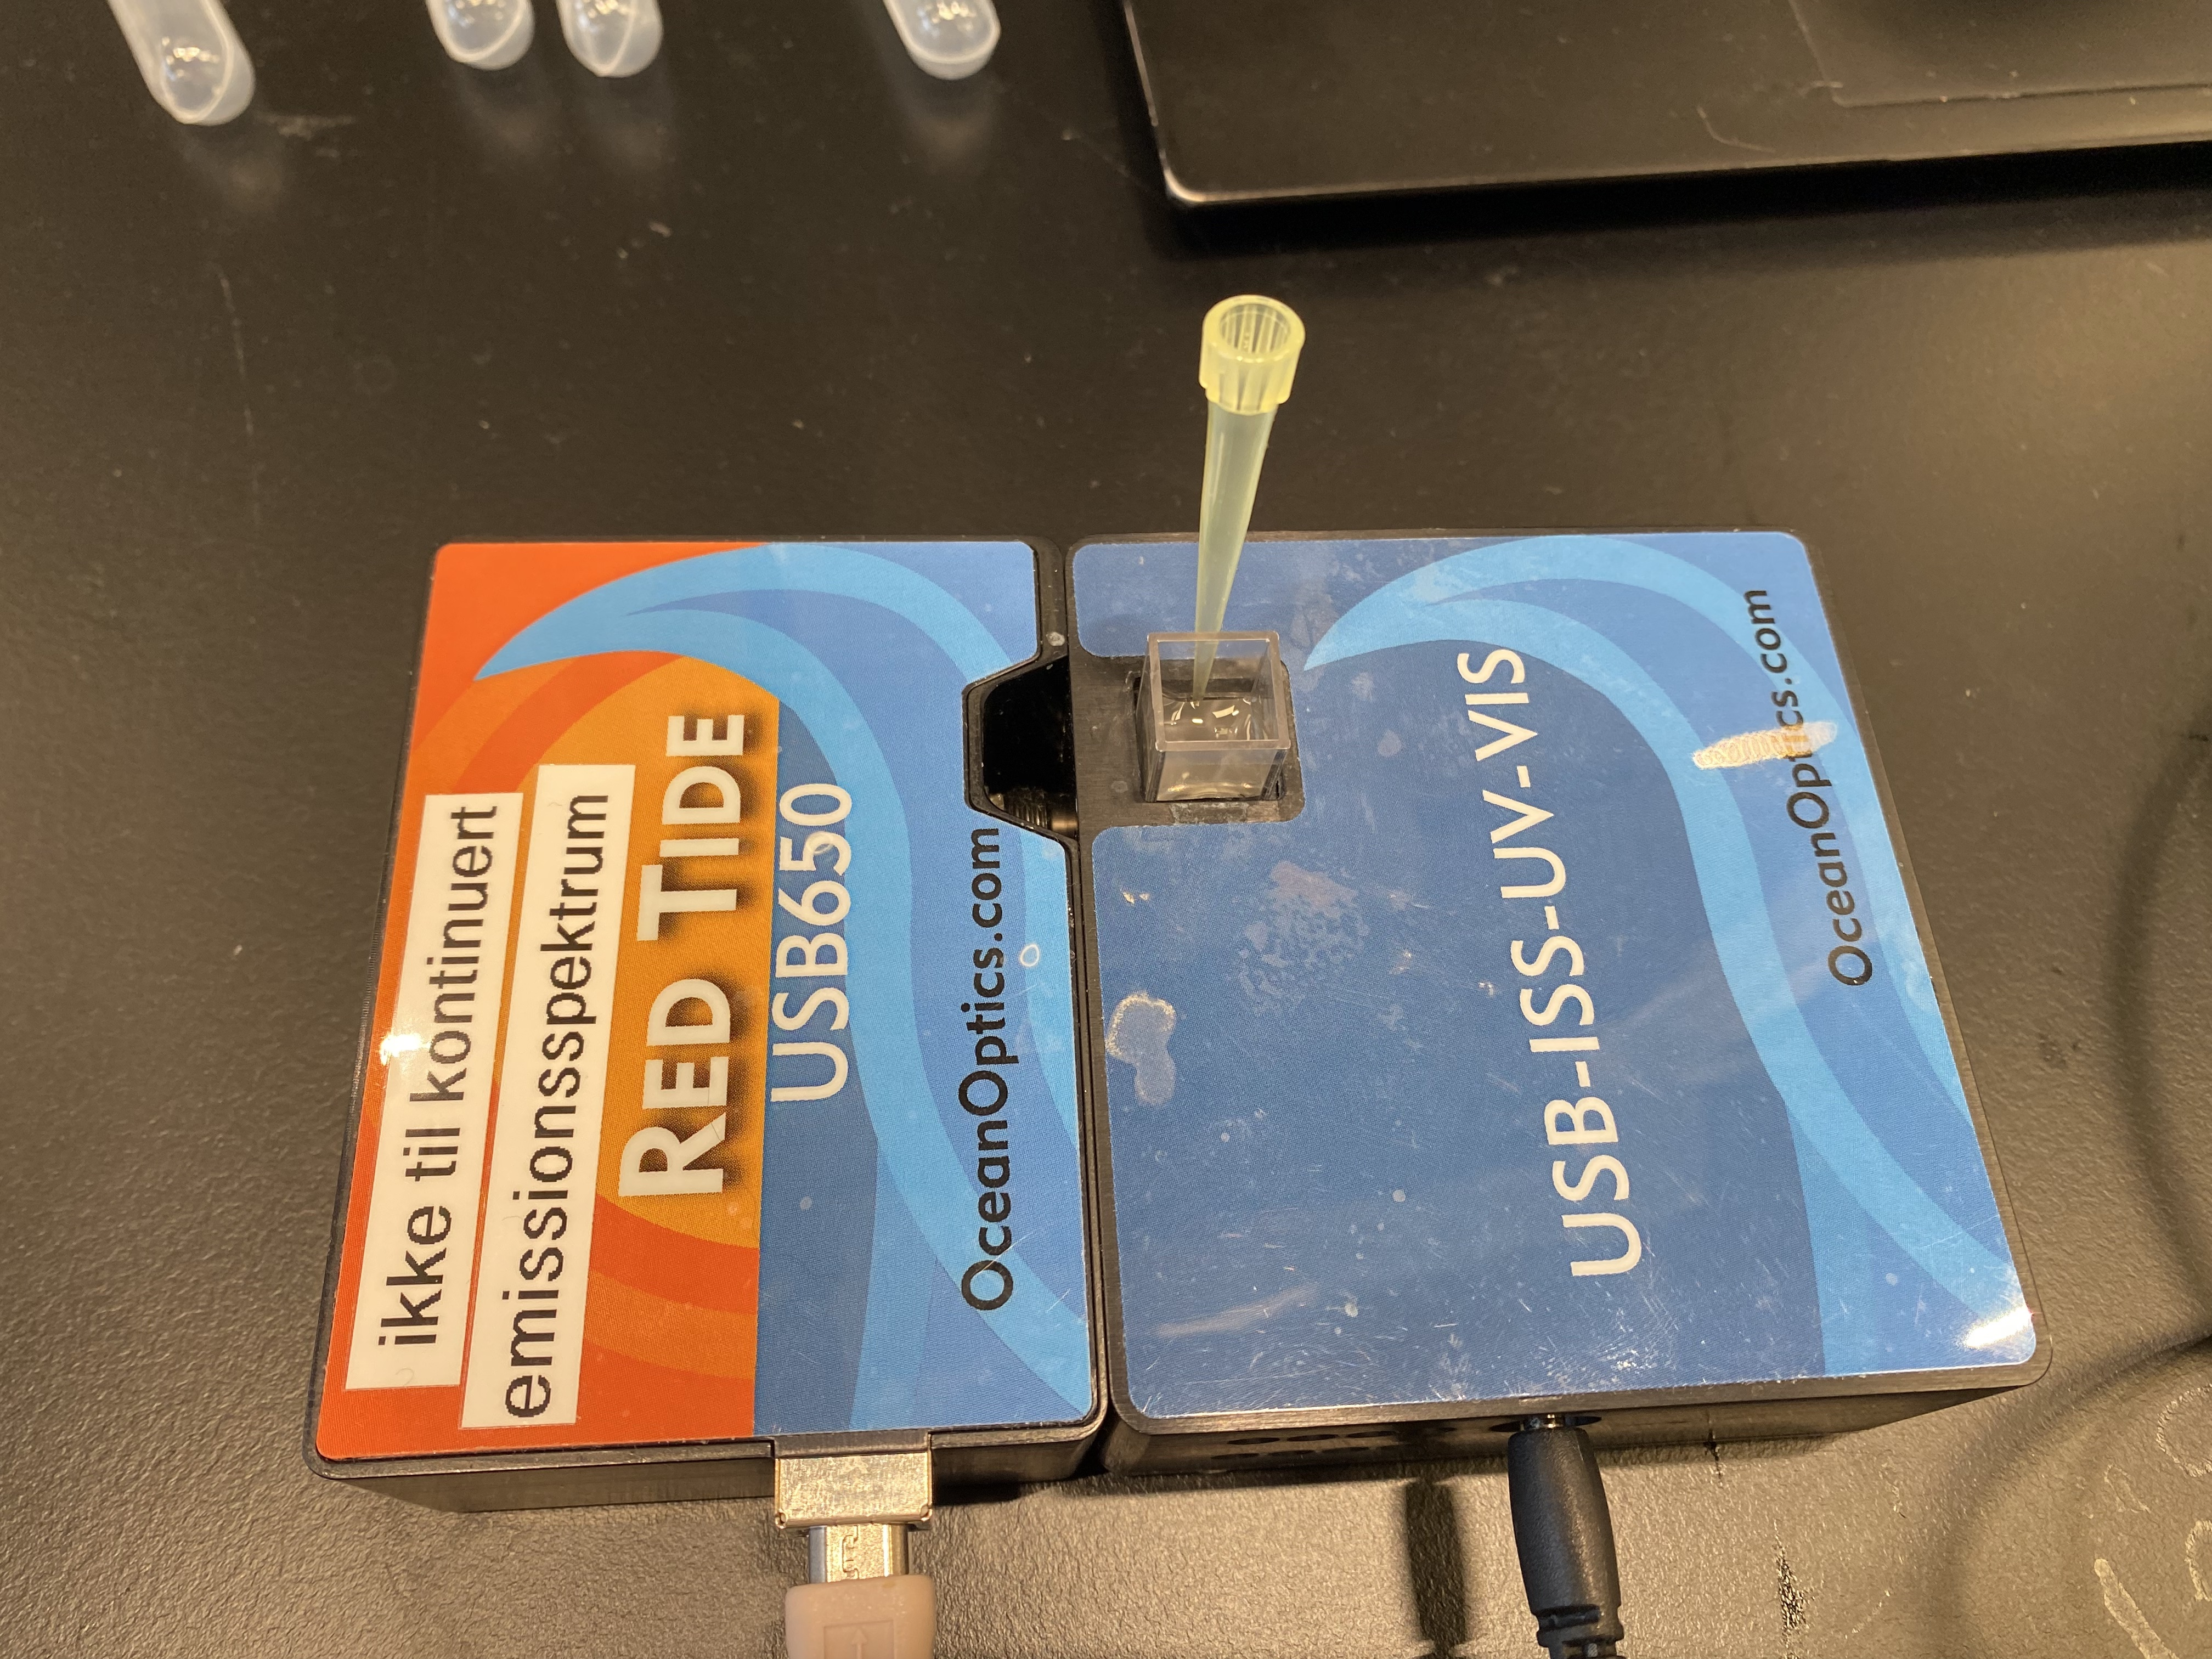
\includegraphics[width=0.6\textwidth]{spektro.jpg}
\end{center}
\caption{Kuvette med opløsning i spektrofotometeret}
\label{fig:spektro}
\end{figure}
\begin{figure}[H]
\begin{center}
  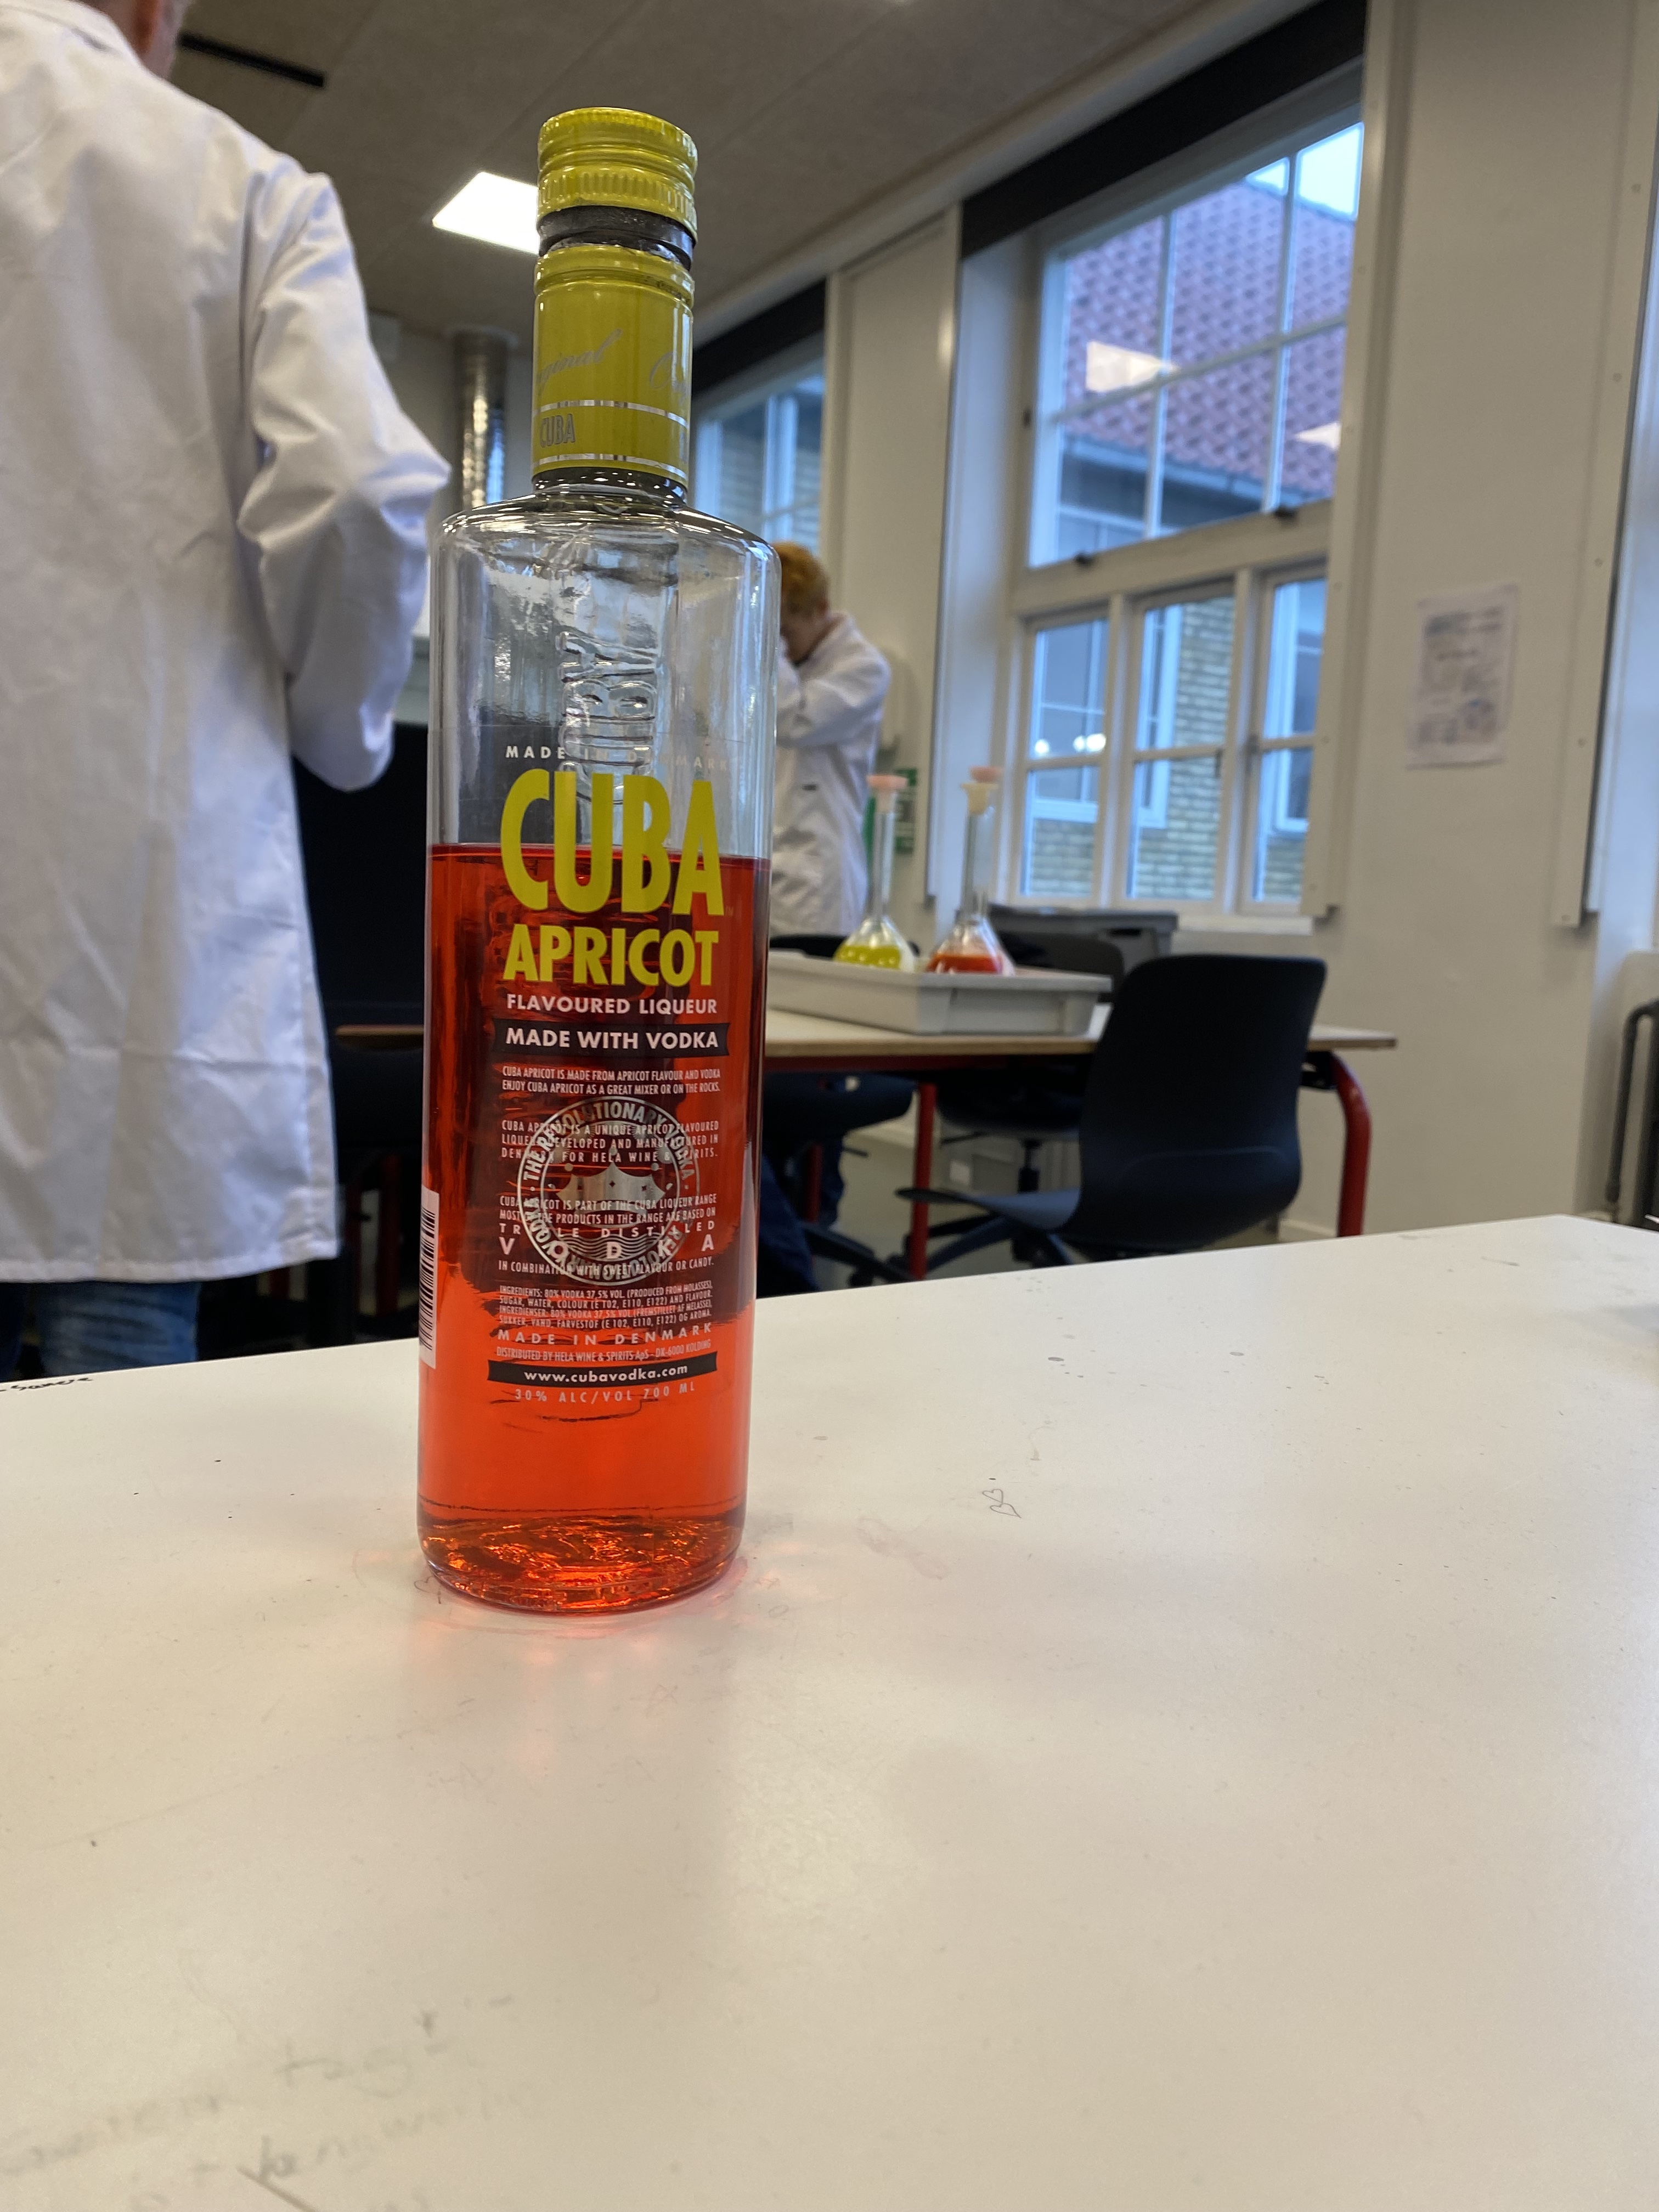
\includegraphics[width=0.5\textwidth]{vodka.jpg}
\end{center}
\caption{En flaske med Cuba Apricot Vodka}
\label{fig:vodka}
\end{figure}
\begin{figure}[H]
\begin{center}
  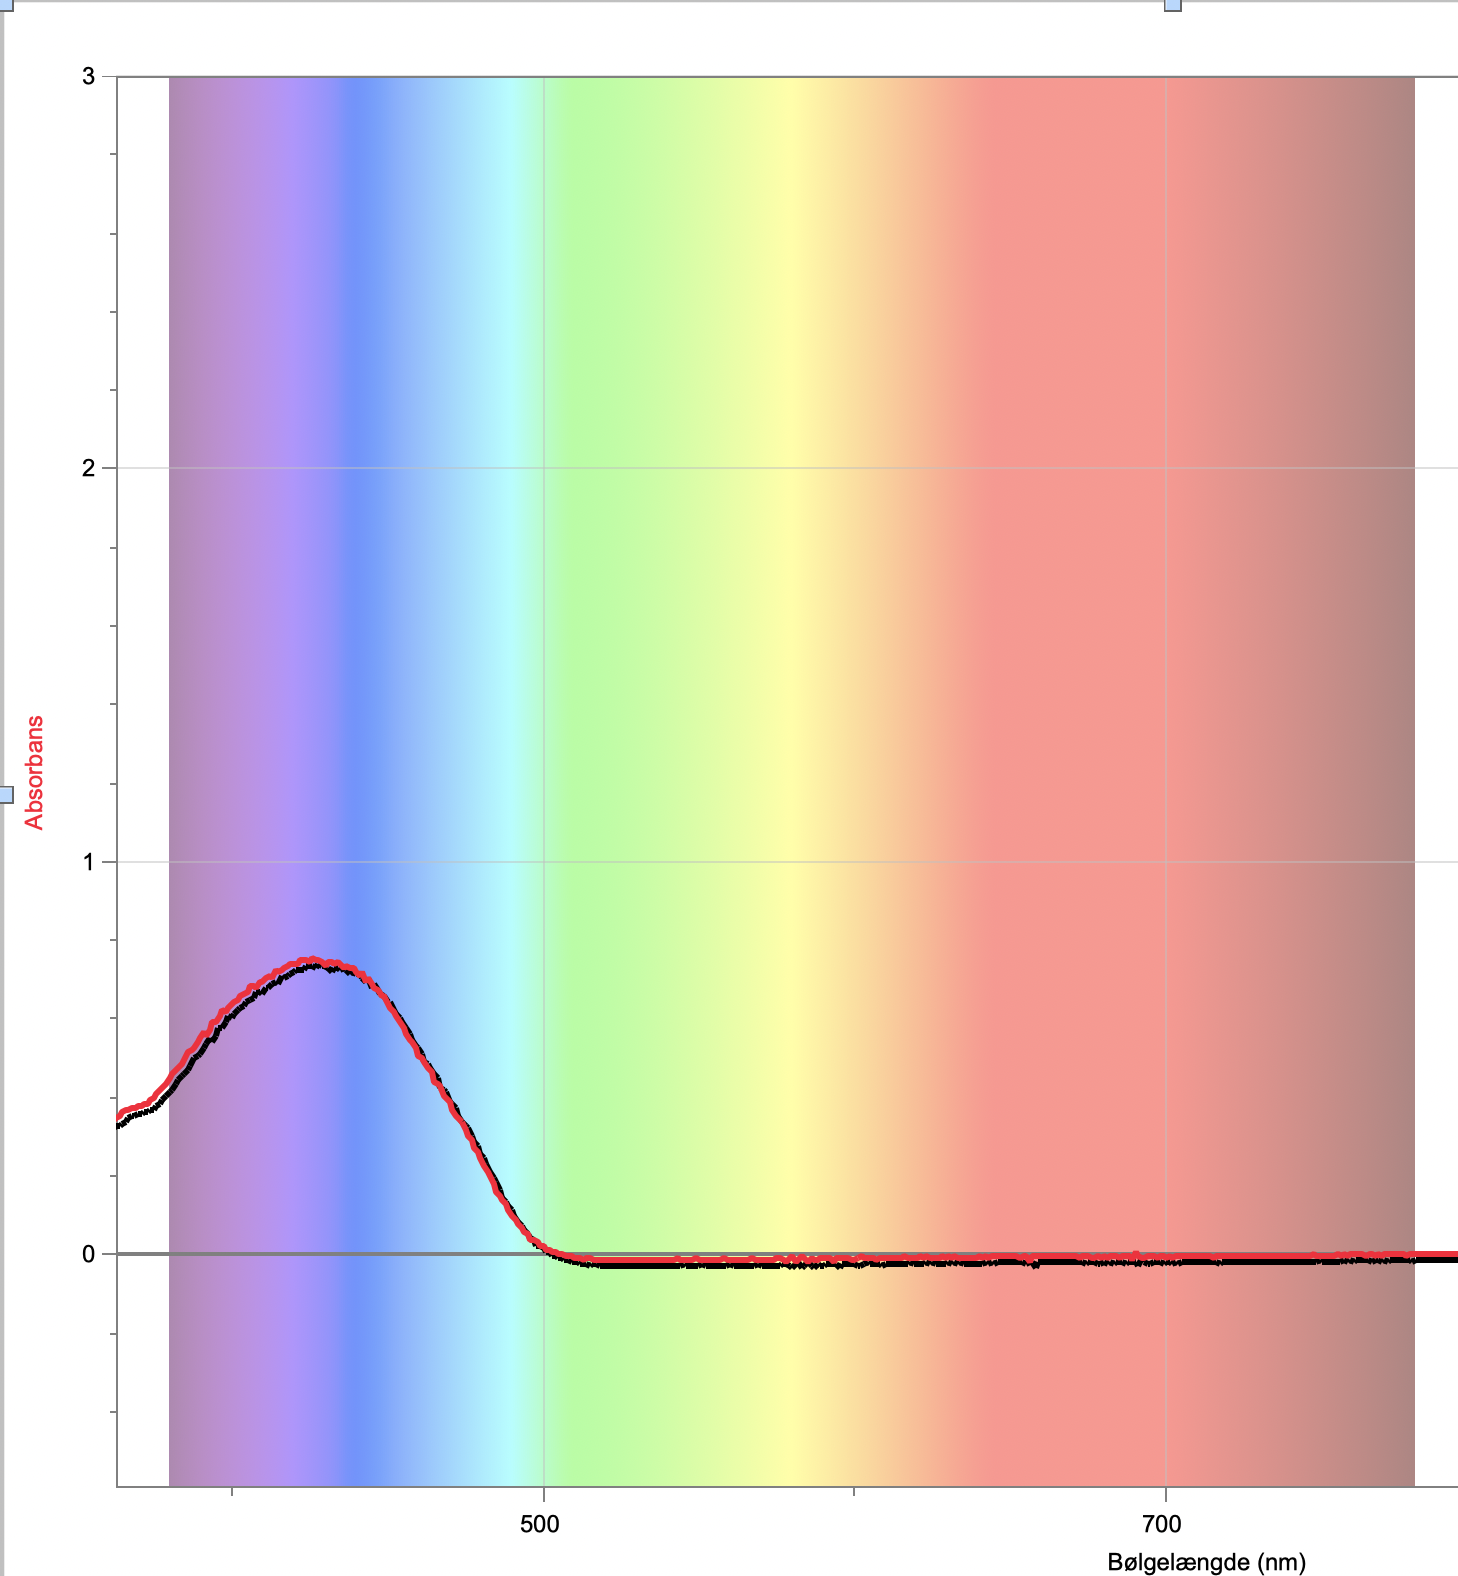
\includegraphics[width=\textwidth]{absorption.png}
\end{center}
\caption{Absorptionsspektrum for tartrazin}
\label{fig:absorption}
\end{figure}


\section{Resultater}
\subsection{Spektrum for atomar hydrogen}
Vi har optaget spektret for atomar hydrogen både fotografisk gennem et gitter som i \cref{fig:spektrum} og via et spektrofotometer som i \cref{fig:spektrum2}.
\begin{figure}[H]
\begin{center}
  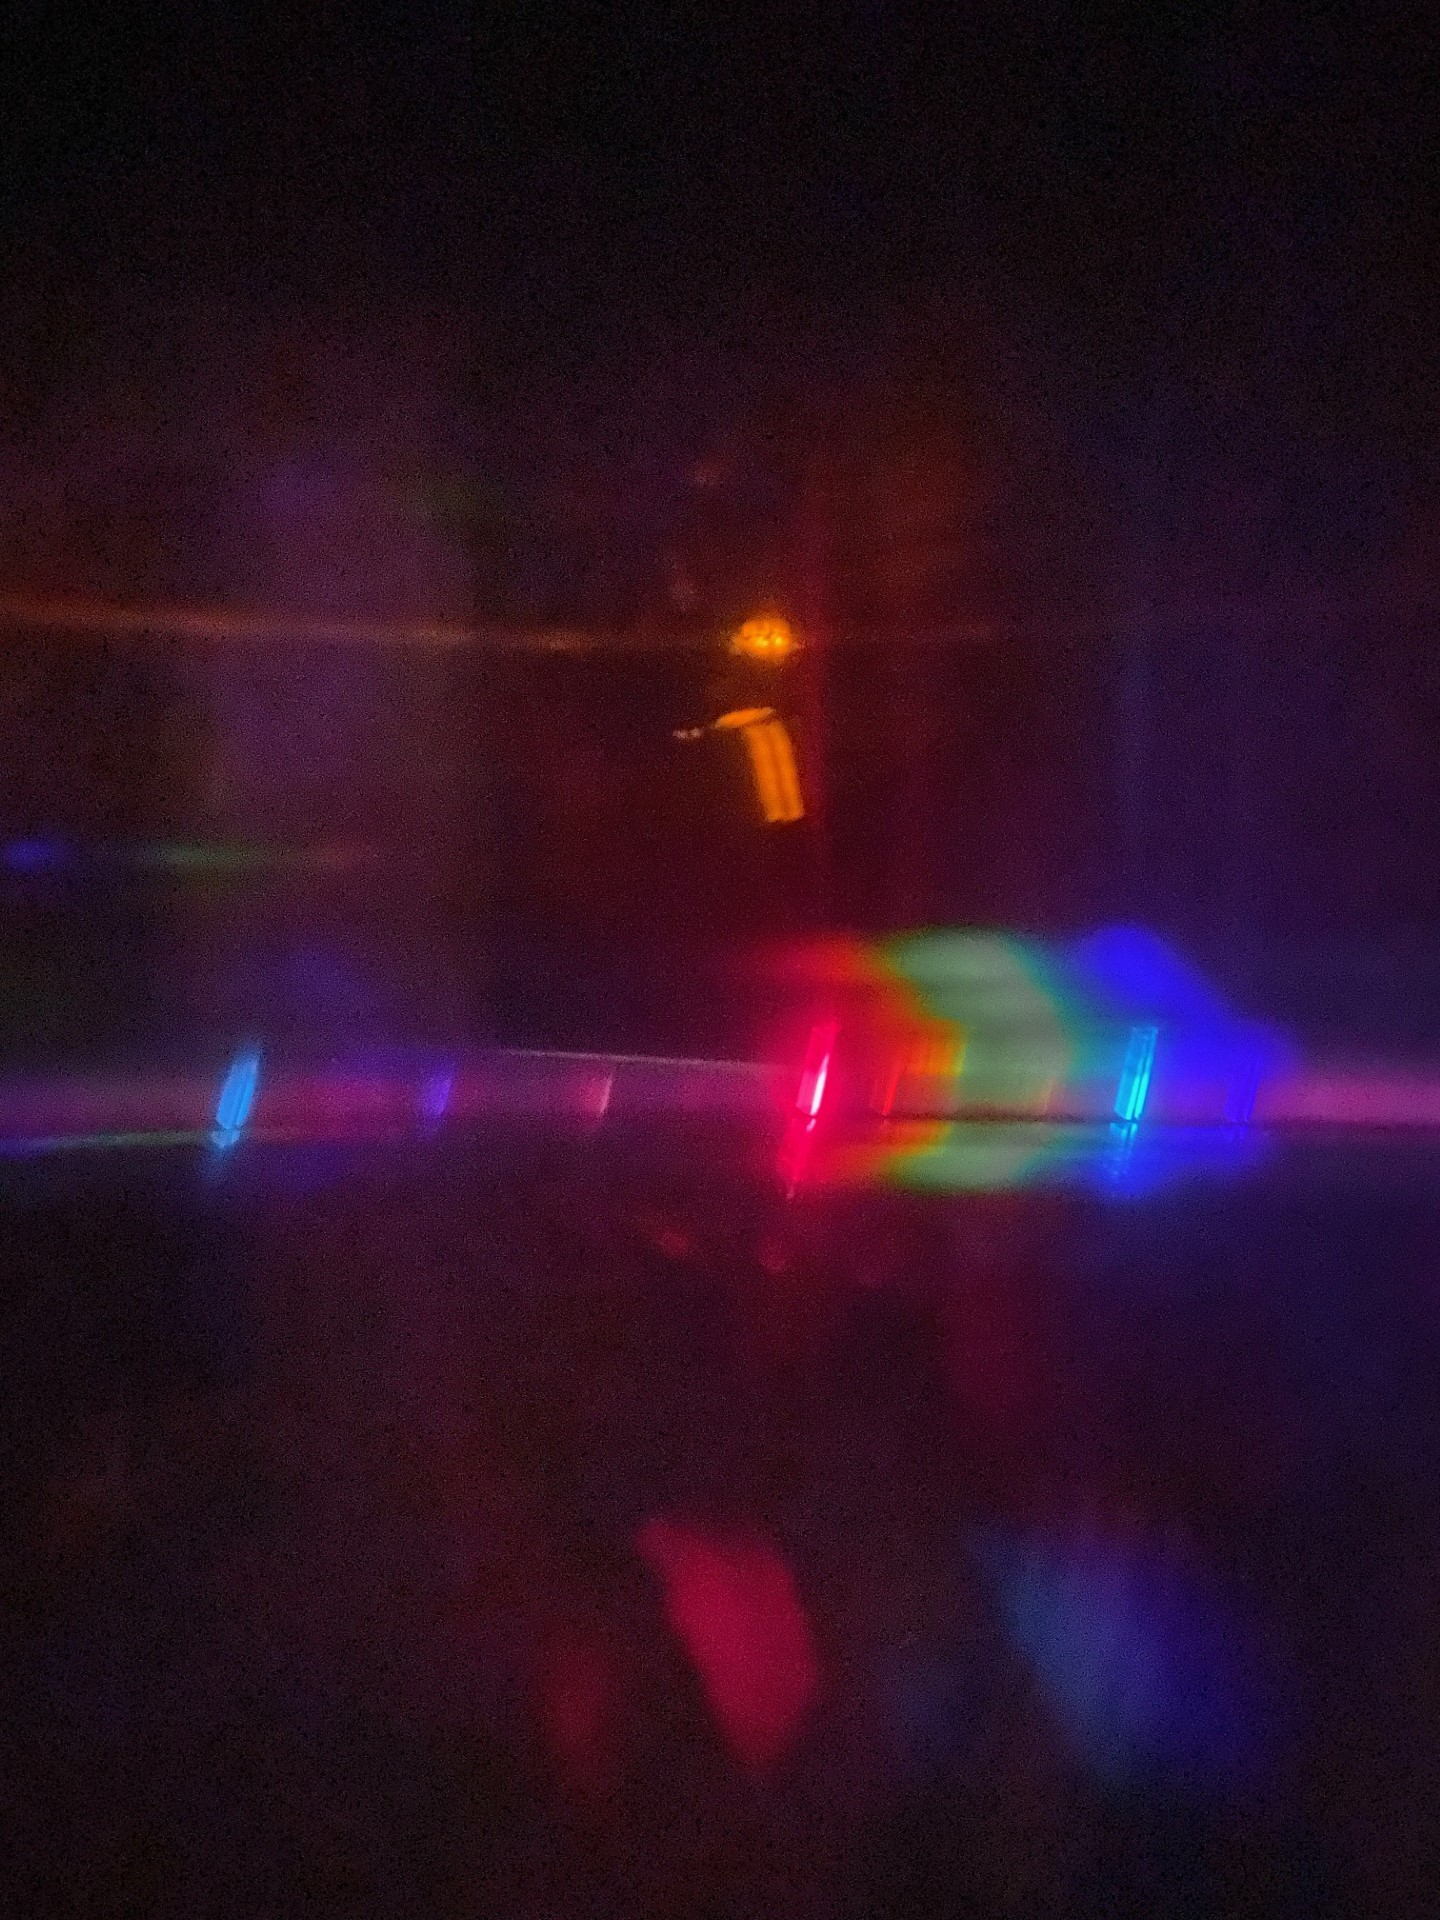
\includegraphics[width=0.7\textwidth]{spektrum.jpeg}
\end{center}
\caption{Spektrum for hydrogen taget fotografisk gennem et gitter}
\label{fig:spektrum}
\end{figure}
\begin{figure}[H]
\begin{center}
  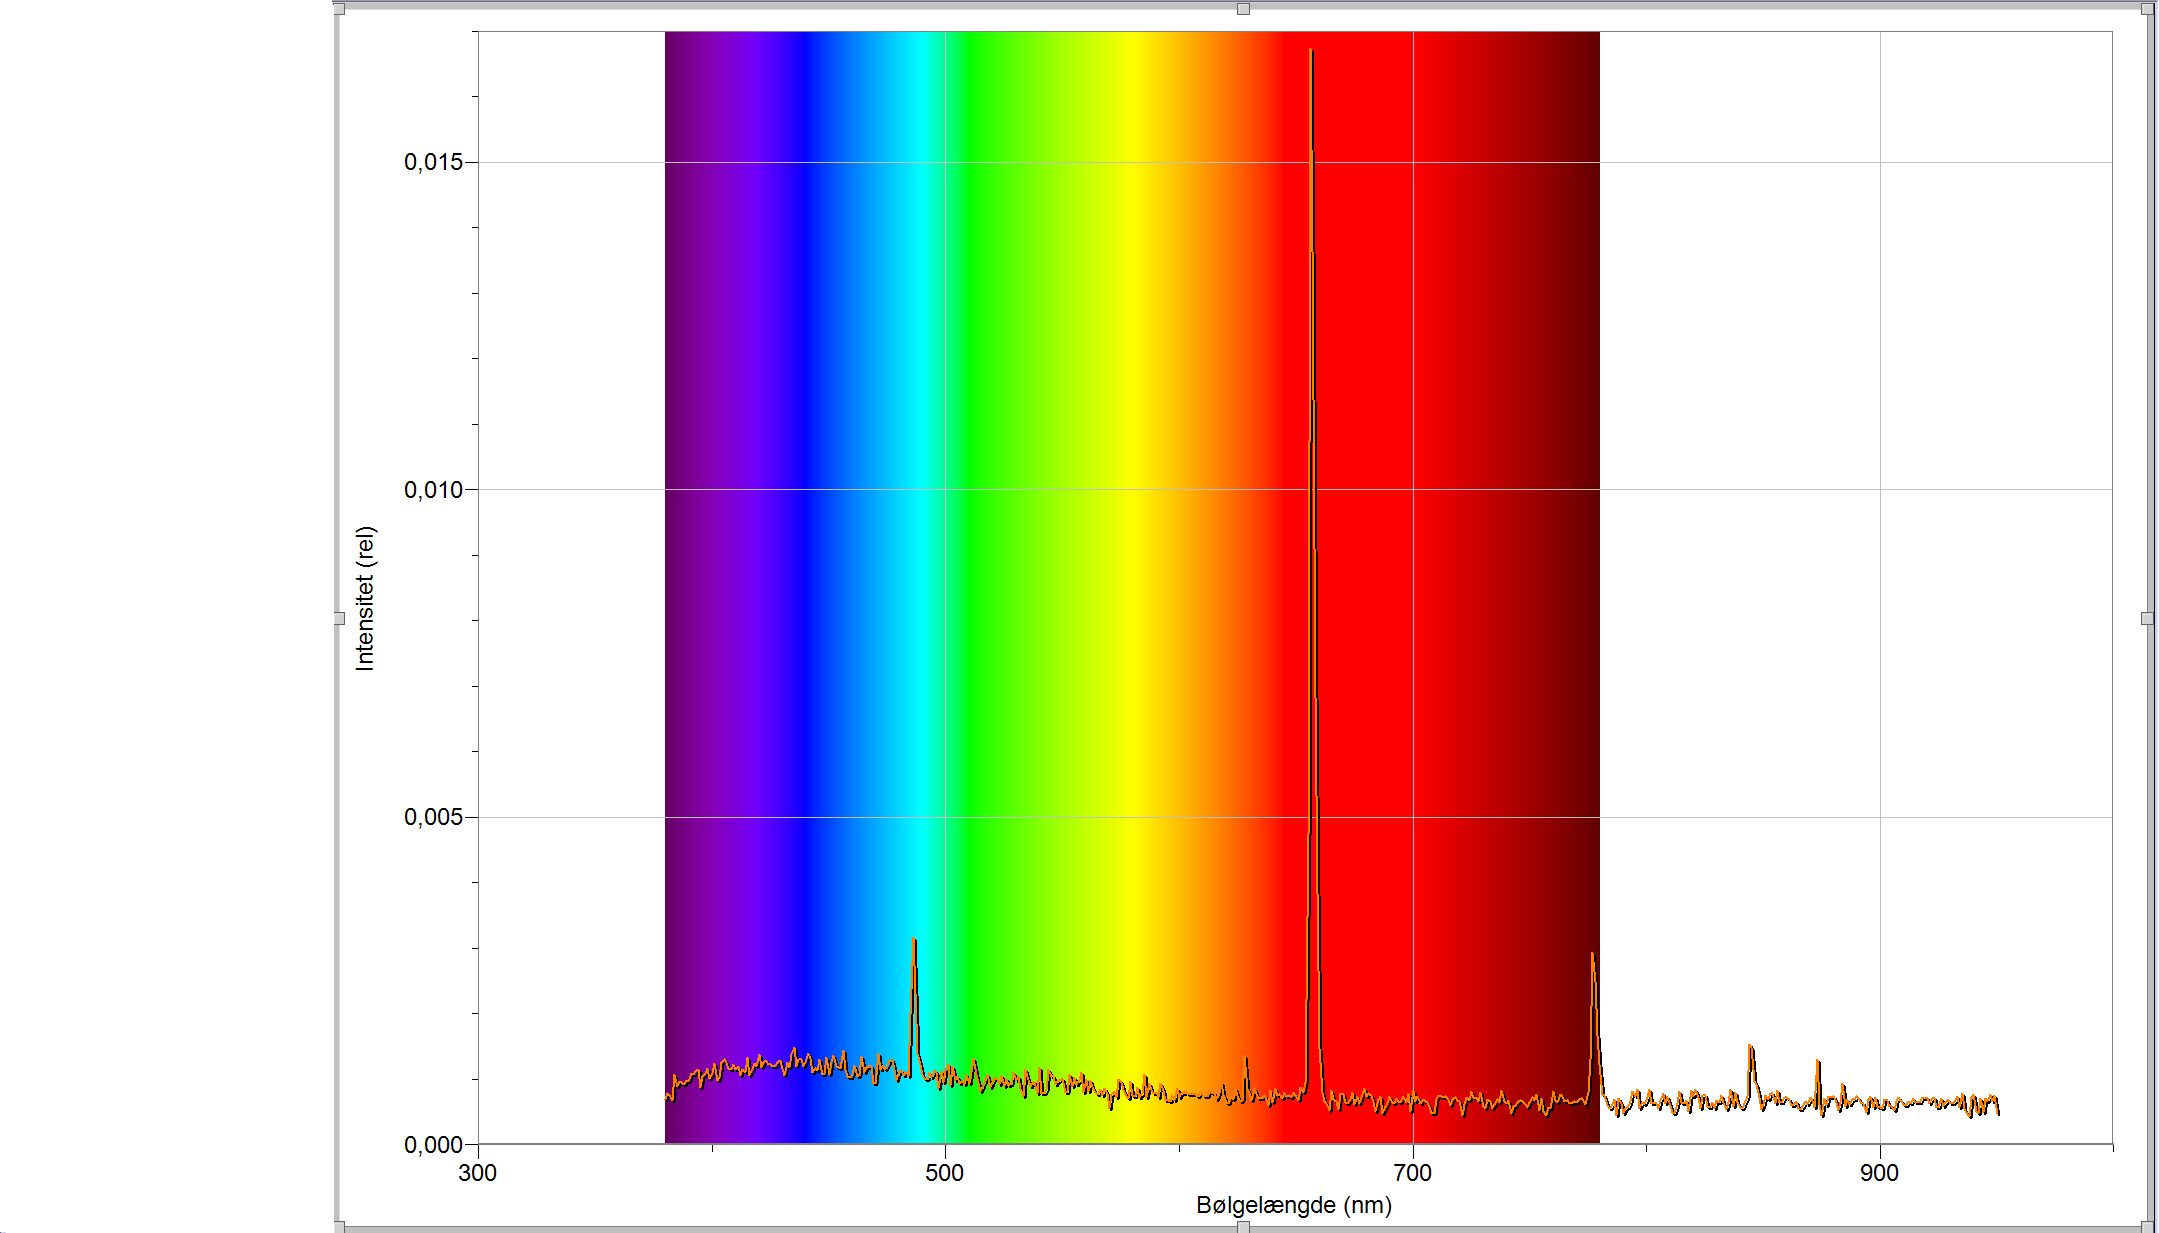
\includegraphics[width=\textwidth]{spektrum2.png}
\end{center}
\caption{Spektrum for hydrogen i LoggerPro taget med et spektrofotometer}
\label{fig:spektrum2}
\end{figure}

\subsection{Bestemmelse af koncentrationerne af farvestoffer i vodka}
Azorubin betegnes med $a$, sunset yellow betegnes med $s$ og tartrazin betegnes med $t$.
$\lambda_{\text{farvestof}}$ betegner bølgelængden, hvor absorbansen for farvestoffet er højest.  
Derudover betegner $k_{\lambda}^{\text{farvestof}}$ konstanten $k_{\lambda}$ ved bølgelængden $\lambda$ for farvestoffet. 

Standardkurverne for tartrazin ses på \cref{fig:stand_kurve}, hvor absorbanserne for standardopløsninger af tartrazin med koncentrationerne set i tabel \ref{tab:kon} ved de tre bølgelængder, hvor absorbansen er maksimal for de tre farvestoffer, er vist.
Standardkurver er også blevet lavet for de to andre farvestoffer, men er udeladt her. 
Hældningskoefficienterne for standardkurverne er da konstanterne $k_{\lambda}^{\text{farvestof}}$ i tabel \ref{tab:abs}.
\begin{table}[H]
\centering
\begin{tabular}{@{}lllll@{}}
\toprule
  \multicolumn{1}{c}{$\lambda_{max}$} & \multicolumn{1}{c}{$A_{\text{vodka}}$} & \multicolumn{1}{c}{Azorubin} & \multicolumn{1}{c}{Sunset Yellow} & \multicolumn{1}{c}{Tartrazin} \\ \midrule
          $\lambda_a = 515 \;\unit{nm} $ & $A(\lambda_a)=0,490$ & $k_{\lambda_a}^{a}=0,0428 \;\unit{L/mg}$ & $k_{\lambda_a}^{s}=0,03539\;\unit{L/mg}$ & $k_{\lambda_a}^{t}=0,0008034\;\unit{L/mg}$         \\
          $\lambda_s =482 \;\unit{nm} $ &  $A(\lambda_s)=0,530$ & $k_{\lambda_s}^{a}=0,0323 \;\unit{L/mg}$&  $k_{\lambda_s}^{s}=0,05204\;\unit{L/mg}$ & $k_{\lambda_s}^{t}=0,01245\;\unit{L/mg}$       \\
          $\lambda_t =429 \;\unit{nm} $ & $A(\lambda_t)=0,669$  & $k_{\lambda_t}^{a}=0,0120 \;\unit{L/mg}$ &  $k_{\lambda_t}^{s}=0,02316\;\unit{L/mg}$ &  $k_{\lambda_t}^{t}=0,03984\;\unit{L/mg}$      \\ \bottomrule
\end{tabular}
\caption{Bølgelængderne, hvor absorbansen er maksimal, absorbanserne for vodkaen ved disse bølgelængder og konstanterne.}
  \label{tab:abs}
\end{table}
\begin{figure}[H]
\begin{center}
  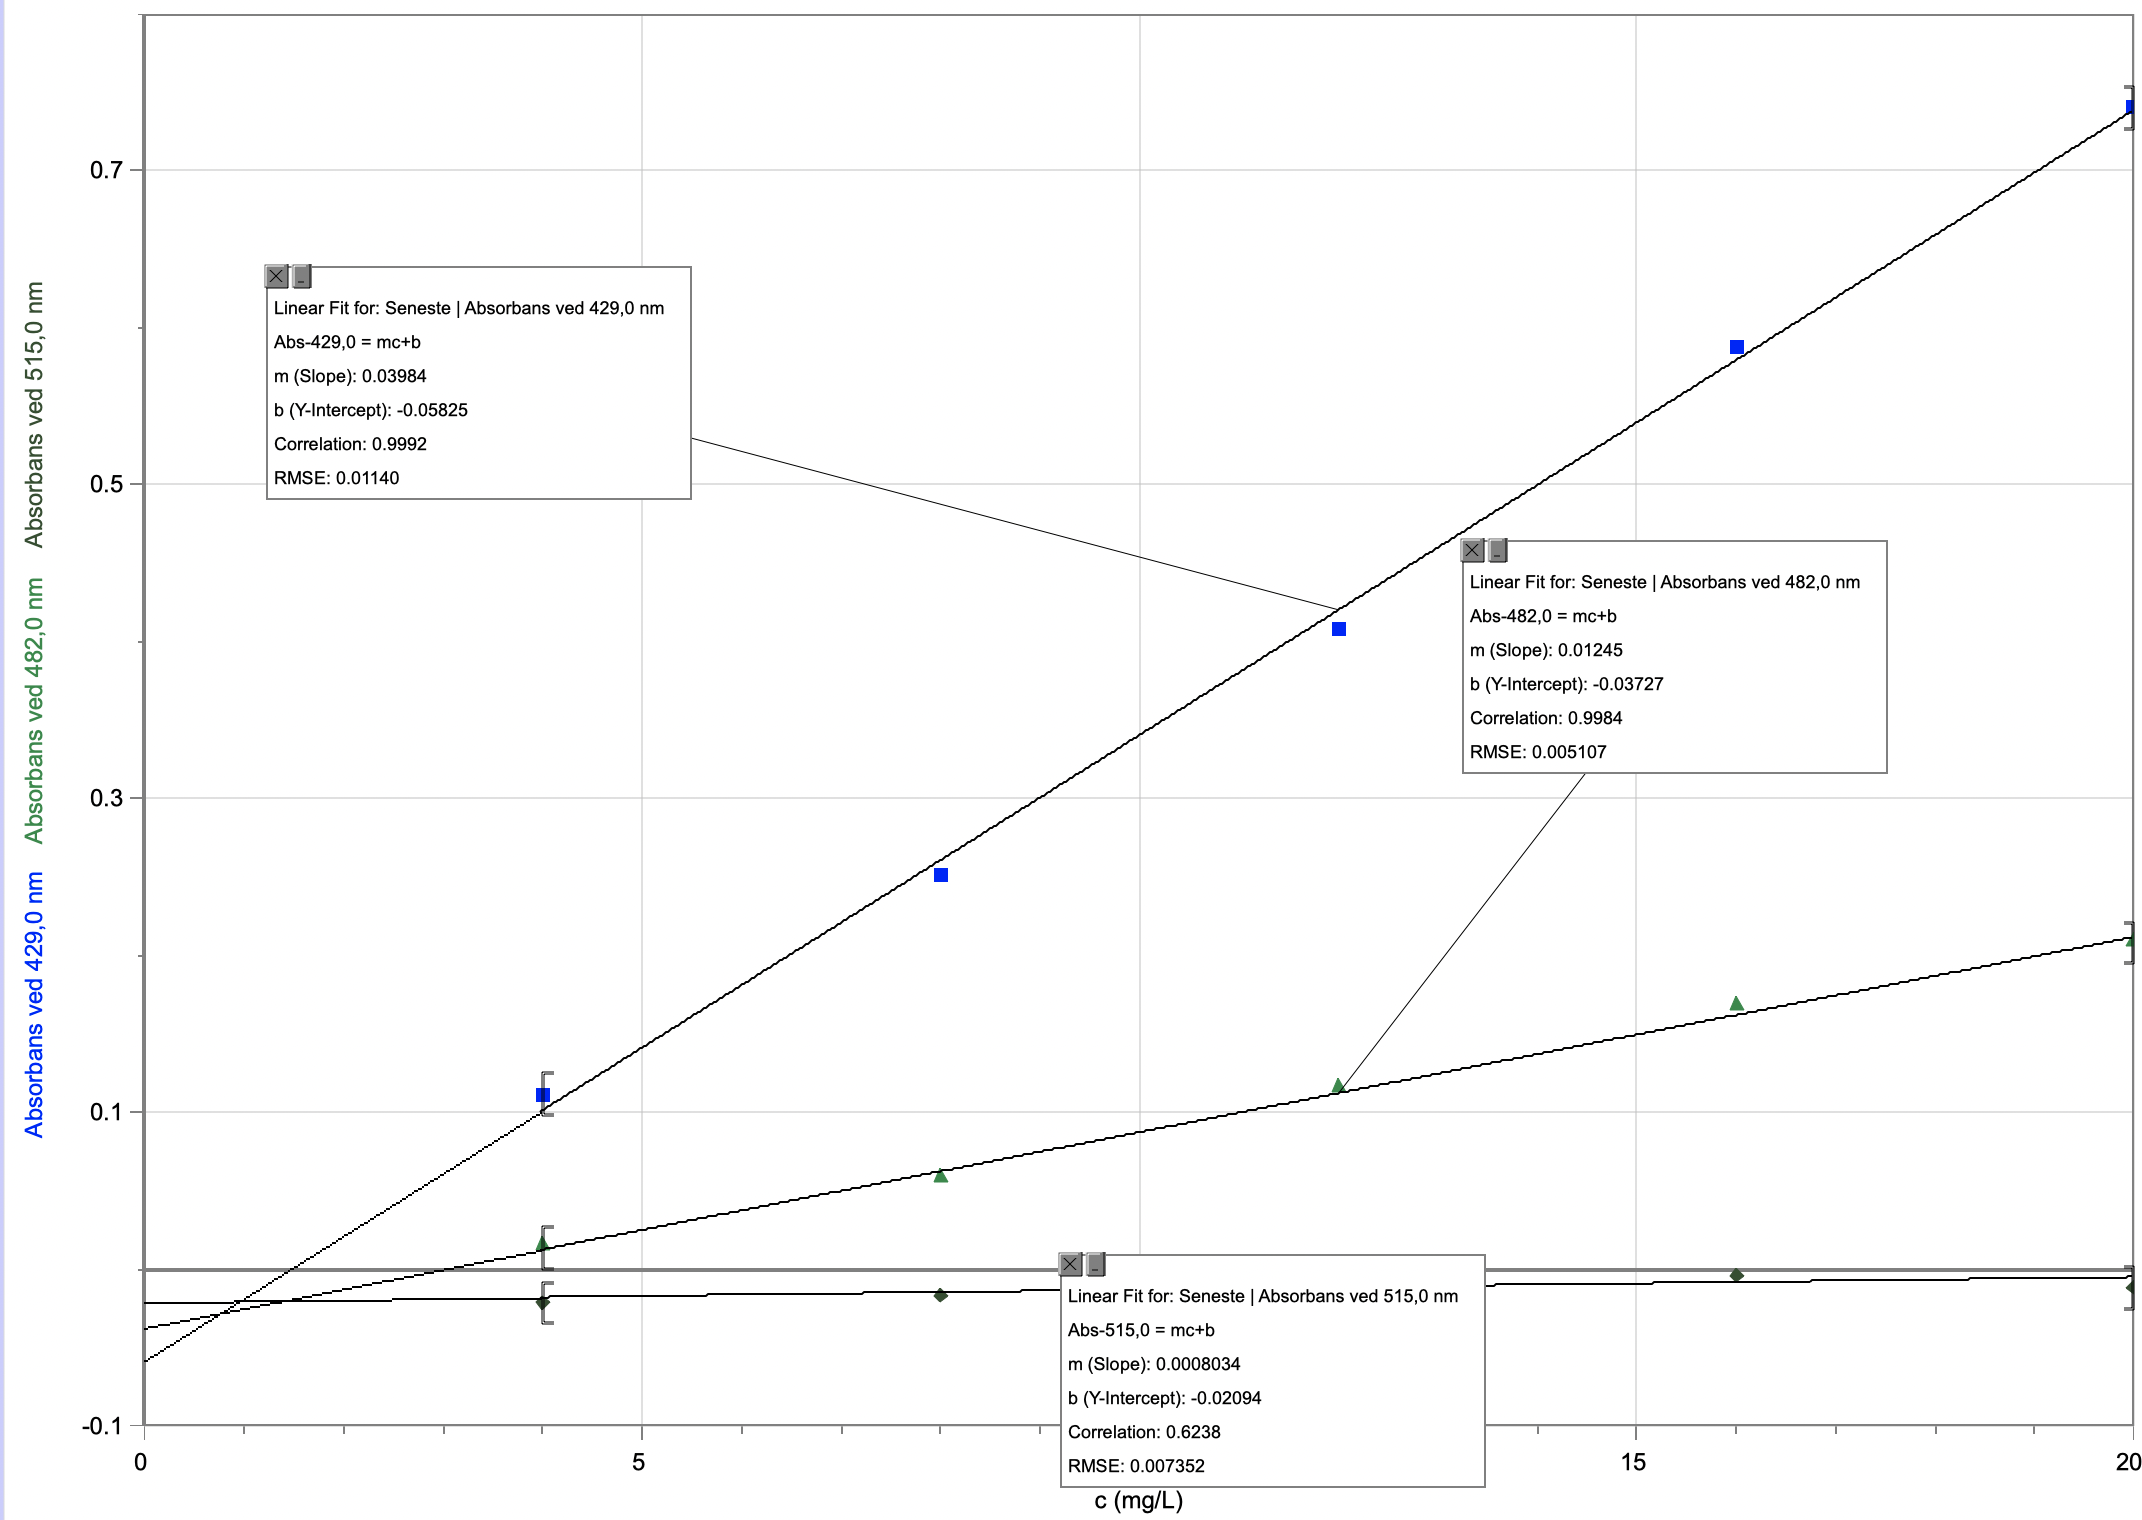
\includegraphics[width=\textwidth]{stand_kurve.png}
\end{center}
\caption{Standardkurverne for tartrazin}
\label{fig:stand_kurve}
\end{figure}

\section{Efterbehandling og diskussion}
\subsection{Spektrum for atomar hydrogen}
Via LoggerPro fandt vi bølgelængderne for linjerne, hvilket kan ses i \cref{fig:top}.
Bemærk at der i stedet for \textit{opbevaringstid (min)} skal stå \textit{bølgelængde }(\unit{nm}).
Lad os nu sammenligne spektret for hydrogen med det for enkeltioniseret helium og dobbelt-ioniseret lithium.

Enkeltioniseret helium og dobbelt-ioniseret lithium er begge hydrogenlignende, siden de begge kun indeholder én elektron.
Energiniveauerne for disse kan ses i \cref{fig:energiniveau}.
Vi ser da, at energierne for nogle af tilstandene er ens for \ce{H} og \ce{He+} samt \ce{H} og \ce{Li^2+}.
Siden forskellen på nogle af disse energier er ens for dem, vil det sige, at der er et sammenfald mellem nogle af linjerne i disses spektre.
Grunden til, at nogle af energierne for tilstandene er ens, som er årsagen til sammenfaldet mellem nogle linjer i spektrene, kan findes i teorien i ligning \ref{eq:hyd_lign}:
\[
E_n=\frac{-13,6\cdot Z^2}{n^2}=\frac{-13,6 \;\unit{eV} }{\left(\frac{n}{Z}\right)^2}
\] 
Siden der for \ce{He+} gælder, at $Z=2$, så må energien $E_n$ være den samme som energien for en tilstand for hydrogen præcis når 
\[
n \in \{2m:m  \in \mathbb{N}\}
\] 
På samme vis gælder der for \ce{Li^2+}, at $Z=3$. Altså må energien $E_n$ være den samme som energien for en tilstand for hydrogen præcis når 
\[
n \in \{3m:m \in \mathbb{N} \}
\] 
\begin{figure}[H]
\begin{center}
  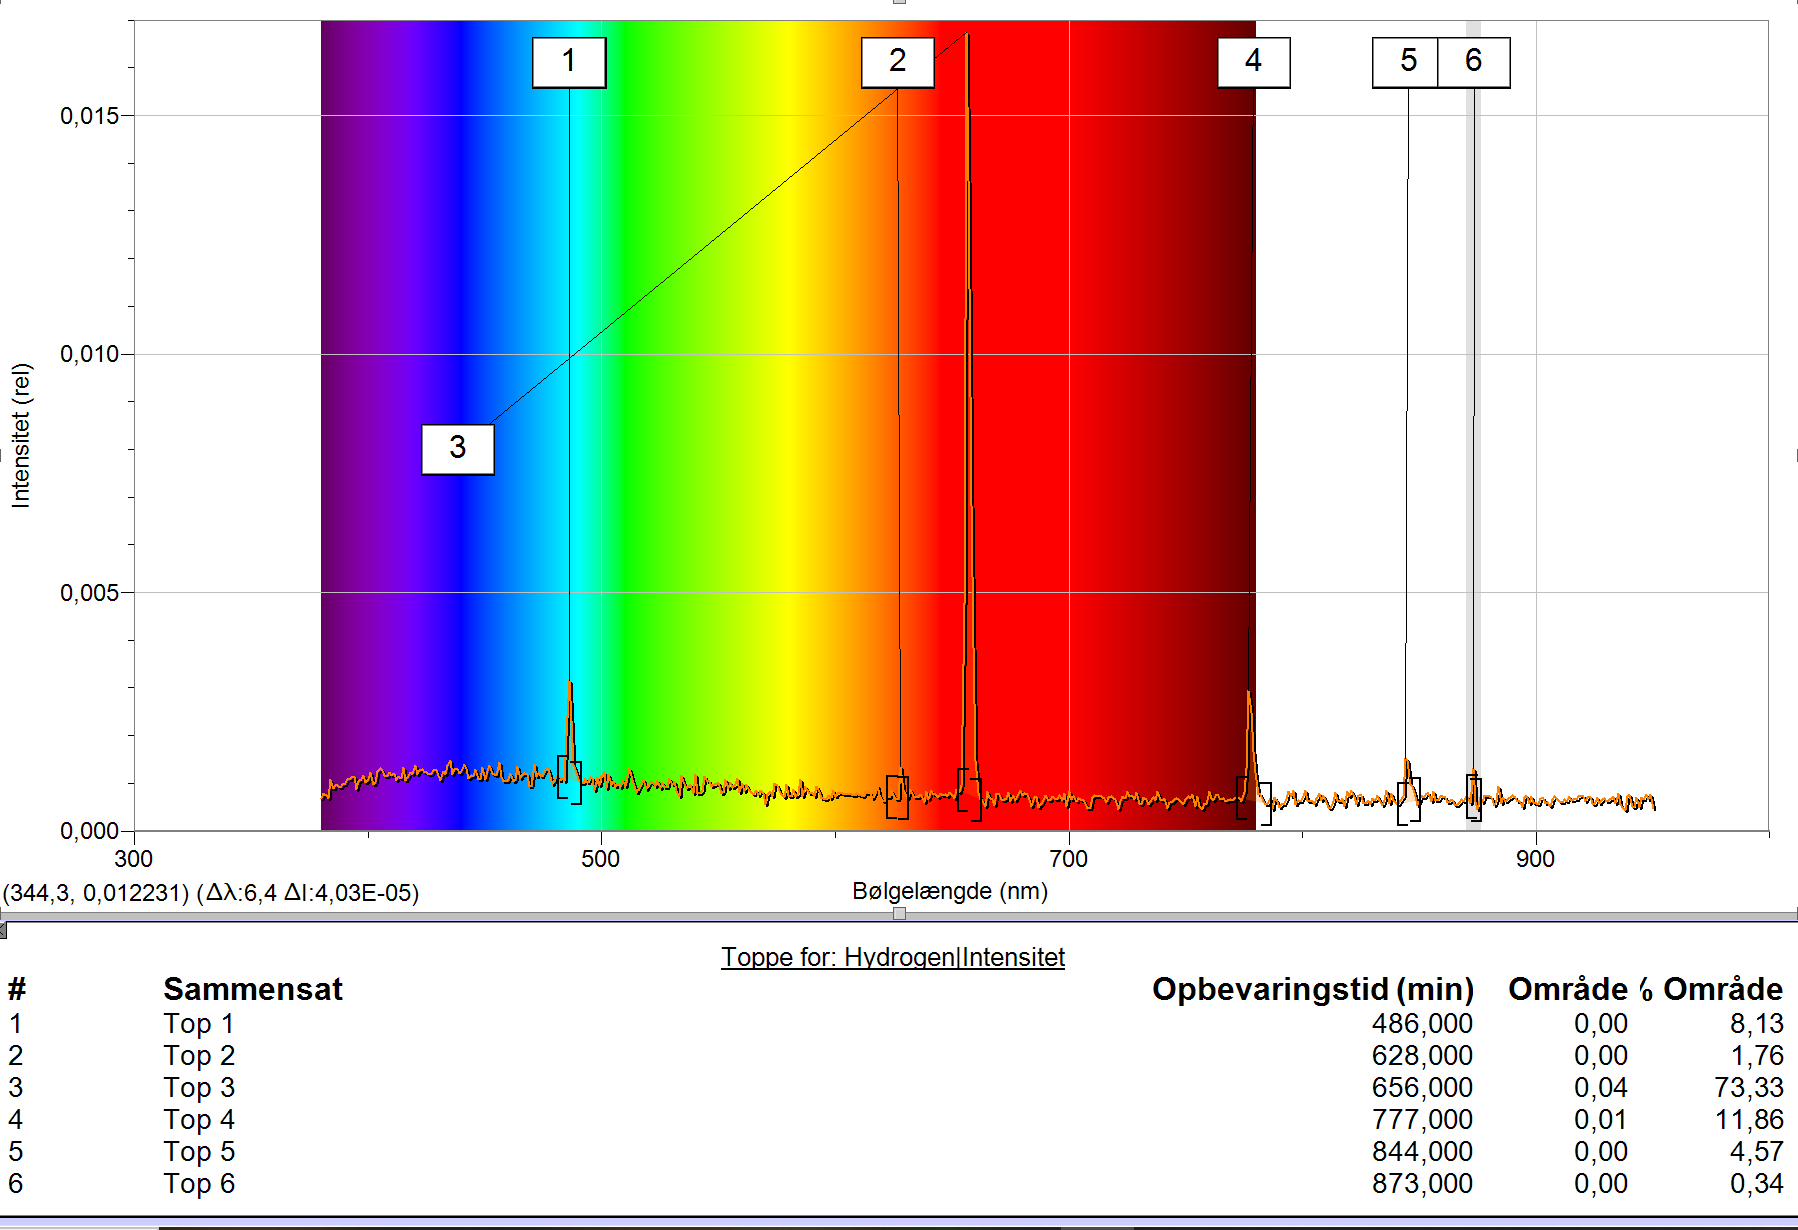
\includegraphics[width=\textwidth]{top.png}
\end{center}
  \caption{Bølgelængderne for linjerne i hydrogenspektret (ikke opbevaringstid)}
\label{fig:top}
\end{figure}
\begin{figure}[H]
\begin{center}
  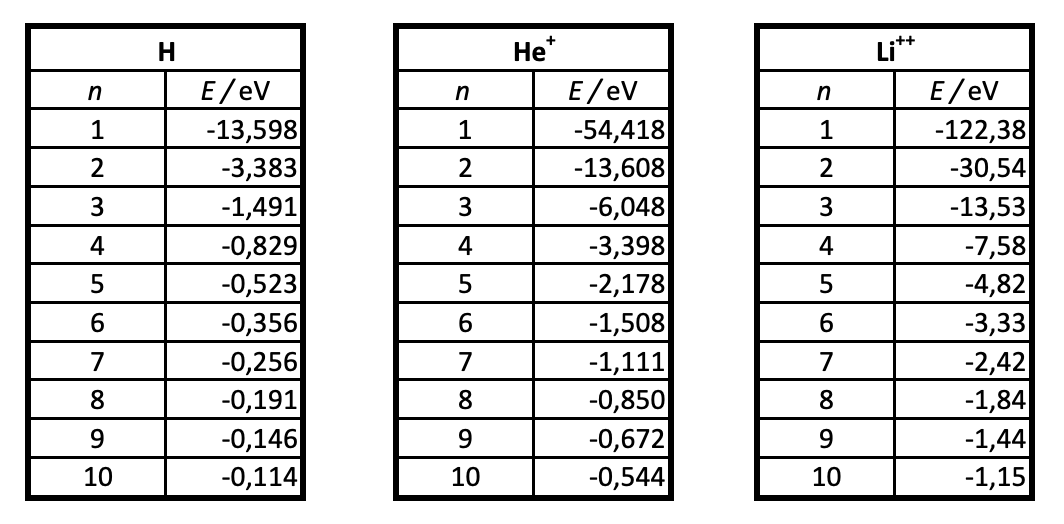
\includegraphics[width=\textwidth]{energiniveau.png}
\end{center}
\caption{Energiniveauerne \ce{H}, \ce{He+} og \ce{Li^2+}}
\label{fig:energiniveau}
\end{figure}

\subsection{Bestemmelse af koncentrationerne af farvestoffer i vodka}
Vores måleresultater er i overensstemmelse med Lambert-Beers lov, da graferne i \cref{fig:stand_kurve} fortæller, at koncentrationen og absorbansen er ligefrem proportionale, siden linjerne bestemt via mindste kvadraters metode tilnærmelsesvis går gennem $(0,0)$.
Årsagen til den negative absorbans når koncentrationen er tæt på $0$, er med stor sandsynlighed grundet sollys og lys fra lamperne i rummet, der ville øge lysintensiteten målt af detektoren i spektrofotometeret. 
Dette er den vigtigste fejlkilde i eksperimentet.

For at bestemme koncentrationerne koncentrationen af azorubin, sunset yellow og tartrazin i vores Cuba Apricot Vodka, udnytter vi additiviteten af absorbansbidragende for hvert enkelt absorberende stof i opløsningen (se Teori).
Vi bruger størrelserne fra tabel \ref{tab:abs} til at opstille tre ligninger med tre ubekendte:
\begin{equation*}
\begin{split}
    0,0428\cdot x + 0,03539 \cdot y + 0,0008034\cdot z&=0,490 \\
 0,0323\cdot x + 0,05204\cdot y + 0,01245\cdot z&=0,530 \\
 0,0120\cdot x + 0,02316\cdot y + 0,03984\cdot z&=0,669 
\end{split}
\end{equation*}
Vi får løsningen til cirka at være
\[
x \approx11,1 \land y \approx0,0593\land z\approx13,4
\] 
Altså vil det sige at
\begin{equation*}
\begin{split}
  c(a)&\approx11,1 \;\unit{mg/L} \\ 
  c(s)&\approx 0,0593 \;\unit{mg/L} \\ 
  c(t)&\approx 13,4 \;\unit{mg/L}
\end{split}
\end{equation*}
Vi har nu bestemt koncentrationerne for azorubin, sunset yellow og tartrazin i vores Cuba Apricot Vodka.
\section{Konklusion}
I denne opgave har vi kigget på Bohrs atommodel og brugt den til at forklare sammenfaldet mellem nogle af linjerne i spektrene for hydrogen, enkeltioniseret helium og dobbelt-ioniseret lithium.
Vi optog et spektrum af hydrogen både fotografisk gennem et gitter og med et spektrofotometer.
Vi brugte også et spektrofotometer til at måle absorbanserne ved bestemte bølgelængder for nogle standardopløsninger af azorubin, sunset yellow og tartrazin, som vi redegjorde for at være farvede.
Vi så, at resultaterne var i overensstemmelse med Lambert-Beers lov.
Derefter målte vi absorbanserne ved nogle bølgelængder for en Cuba Apricot Vodka, og benyttede så den additive egenskab ved de individuelle absorbansbidrag fra hvert enkelt absorberende stof til at finde koncentrationerne af de tre farvestoffer i vodkaen.
Vi fandt koncentrationen af azorubin til at være $11,1 \;\unit{mg/L} $, koncentrationen af sunset yellow til at være $0,0593 \;\unit{mg/L} $ og koncentrationen af tartrazin til at være $13,4 \;\unit{mg/L} $. 
%%%%%%%%%%%%%%%%%%%%%%% BIBLIOGRAPHY %%%%%%%%%%%%%%%%%%%%%%%

\newpage
\singlespacing %%Makes single spaced
\bibliographystyle{apa-good} %%bib style found in bst folder, in bibtex folder, in texmf folder.
\setlength{\bibsep}{5pt} %%Changes spacing between bib entries
\bibliography{Zotero} %%bib database found in bib folder, in bibtex folder
\thispagestyle{empty} %%Removes page numbers
\end{document}
